% !TeX encoding = UTF-8
\documentclass[12pt]{article}

\usepackage{setspace}
\usepackage{CJKutf8}
\usepackage{enumitem}
\usepackage{array}
\usepackage{multirow}
\usepackage{amsmath}
\usepackage{graphicx}
\usepackage{subcaption}
\usepackage{setspace}
\usepackage{wallpaper}
\usepackage{adjustbox}
\usepackage{afterpage}
\usepackage{lscape}
\usepackage{mathptmx}
\usepackage{titlesec}
\usepackage{float}
\usepackage[hyphens]{url}
\usepackage[margin=2.8cm]{geometry}
\addtolength{\wpXoffset}{+9.26cm}
\addtolength{\wpYoffset}{-12.5cm}
\usepackage[backend=bibtex]{biblatex}

\bibliography{main}

\usepackage{booktabs}
\usepackage{siunitx} % Required for alignment
\sisetup{
  round-mode = places, % Rounds numbers
  round-precision = 2, % to 2 places
}
\usepackage{listings}
\usepackage{color}
\usepackage{hyperref}
\hypersetup{
    colorlinks,
    citecolor=black,
    filecolor=black,
    linkcolor=black,
    urlcolor=black
}
\renewcommand\lstlistingname{Figure}
\renewcommand\lstlistlistingname{Figures}

\DeclareCaptionLabelFormat{tablel}{#1 #2}
\captionsetup[table]{labelsep=period}
\captionsetup[figure]{labelsep=period}

\lstset{
  language=XML,
  morekeywords={encoding,
  xs:schema,xs:element,xs:complexType,xs:sequence,xs:attribute}
}

\title{Recognizing Chinese Textual Entailment by Deep Learning}
\author{
  Wei-Ting Chen\\
  National Taiwan Ocean University\\
  \texttt{10757025@mail.ntou.edu.tw}\\
  \\
  Chuan-Jie Lin\\
  Nation Taiwan Ocean University\\
  \texttt{cjlin@mail.ntou.edu.tw}\\
}

\titleclass{\subsubsubsection}{straight}[\subsection]

\newcounter{subsubsubsection}[subsubsection]
\renewcommand\thesubsubsubsection{\thesubsubsection.\arabic{subsubsubsection}}
\renewcommand\theparagraph{\thesubsubsubsection.\arabic{paragraph}} % optional; useful if paragraphs are to be numbered

\titleformat{\subsubsubsection}
  {\normalfont\normalsize\bfseries}{\thesubsubsubsection}{1em}{}
\titlespacing*{\subsubsubsection}
{0pt}{3.25ex plus 1ex minus .2ex}{1.5ex plus .2ex}

\makeatletter
\renewcommand\paragraph{\@startsection{paragraph}{5}{\z@}%
  {3.25ex \@plus1ex \@minus.2ex}%
  {-1em}%
  {\normalfont\normalsize\bfseries}}
\renewcommand\subparagraph{\@startsection{subparagraph}{6}{\parindent}%
  {3.25ex \@plus1ex \@minus .2ex}%
  {-1em}%
  {\normalfont\normalsize\bfseries}}
\def\toclevel@subsubsubsection{4}
\def\toclevel@paragraph{5}
\def\toclevel@paragraph{6}
\def\l@subsubsubsection{\@dottedtocline{4}{7em}{4em}}
\def\l@paragraph{\@dottedtocline{5}{10em}{5em}}
\def\l@subparagraph{\@dottedtocline{6}{14em}{6em}}
\makeatother

\setcounter{secnumdepth}{4}
\setcounter{tocdepth}{4}

\begin{document}
  \begin{CJK*}{UTF8}{bkai}

  \begin{titlepage}
  \centering
  {\Huge 國立臺灣海洋大學\par}
  \vspace{1cm}
  {\huge 資訊工程學系\par}
  \vspace{1cm}
  {\huge 碩士學位論文\par}
  \vspace{2cm}
  {\LARGE 指導教授:林川傑\ (Lin, Chuan-Jie) 博士\par}
  \vfill
  {\LARGE 以深度學習辨識中文文本蘊涵關係\par}
  {\LARGE Recognizing Chinese Textual Entailment by Deep Learning\par}
  \vfill
  {\LARGE 研究生:陳威廷\ \bigg(
    \begin{tabular}{c}
      Chen, Wei-Ting \\
      M00000000
    \end{tabular}
    \bigg) 撰}
    \vfill
    {\LARGE 中華民國\ 110 年\ 03 月}
  \end{titlepage}

  \newpage

  \begin{titlepage}
    \centering
  {\LARGE 以深度學習辨識中文文本蘊涵關係\par}
  \vfill
  {\Large Recognizing Chinese Textual Entailment by Deep Learning\par}
  \vfill
  {
    \Large
    \begin{minipage}{2in}
      研究生:陳威廷 \\
      指導教授:林川傑
    \end{minipage}
    \hfill
    \begin{minipage}{2.4in}
      Student: Chen, Wei-Ting \\
      Advisor: Lin, Chuan-Jie
    \end{minipage}
    \par
    }
    \vfill
    {\LARGE 國立臺灣海洋大學\par}
    {\LARGE 資訊工程學系\par}
    {\LARGE 碩士學位論文\par}
    \vfill
    {
      \LARGE
      A Thesis \\
      Submitted to Computer Science and Engineering \\
      Electrical Engineering and Computer Science \\
      National Taiwan Ocean University \\
      In Partial Fulfillment of the Requirements \\
      for the Degree of \\
      Master of Science \\
      in \\
      Computer Science and Engineering \\
      March, 2021 \\ \vspace{0.5cm}
      Keelung, Taiwan, Republic of China
      }
      \vfill
      {\LARGE 中華民國\ 110 年\ 03 月}
\end{titlepage}

\pagenumbering{gobble}

\newpage

\CenterWallPaper{0.1}{ntou.png}
\doublespacing
\tableofcontents
\singlespacing

\newpage

\listoffigures
\listoftables

\newpage

\pagenumbering{arabic}

\newcommand{\PreserveBackslash}[1]{\let\temp=\\#1\let\\=\temp}
\newcolumntype{C}[1]{>{\PreserveBackslash\centering}p{#1}}
\newcolumntype{R}[1]{>{\PreserveBackslash\raggedleft}p{#1}}
\newcolumntype{L}[1]{>{\PreserveBackslash\raggedright}p{#1}}

\titleformat{\section}{\clearpage\centering\normalfont\huge}{Chapter \thesection.}{1em}{}
\begin{spacing}{1.77}
\section{Introduction} \label{section:introduction}

\subsection{Motivation}
\paragraph{}
% NLI 任務在定義上並不複雜,給定一句 Premise 和一句 Hypothesis,並辨識這兩句話是否存在蘊含關係。一個文意蘊含任務的分類有很多種類型,最簡單的分法就是「有蘊含」與「沒有蘊含」,而「沒有蘊含」的部份可以進一步的分成「互斥」與「獨立」,「有蘊含」的部份也可以進一步的分成「正向蘊含」與「雙向蘊含」。去判別兩句話之間是否存在蘊含關係,這個任務的難度會因為涉及的語言現象而產生很高的複雜度
The definition of the textual entailment (also called natural language inference) task is not complex, given a premise sentence and a hypothesis sentence, and recognizing if the two sentences are entailment. The category of the textual entailment tasks has many types, the simplest one is to divide into ``entailment'' and ``not entailment''. Further, ``not entailment'' can be divided into ``contradiction'' and ``independence'', and ``entailment'' can be divided into ``forward entailment'' and ``bi-directional entailment''. The determination of the relation of the two sentences will become highly difficult according to the complexity of the linguistic phenomenon that the sentences involved.

\paragraph{}
% 模型是否能夠精準判別此蘊含關係,是衡量此模型的自然語言理解能力很重要的指標。在許多自然語言的應用中,例如:問答系統、文件摘要、資訊擷取與機器翻譯等,若是能提高模型的語言理解能力,將會是相當有幫助的事情。
Whether a model can accurately inference the relation of the sentences is quite important a indicator to measure the natural language understanding ability of the model. Increasing the NLU ability of the model will be helpful in many applications of the NLP, for example, question-answering system, summarization, information extraction, and machine translation.

\paragraph{}
% 近年來深度學習在 NLI 任務上取得了巨大的成功,但多數的成果都是僅限於大型英文資料集。本論文將會以繁體中文的 NLI 資料集 - RITE 為主要目標,將這份成功帶到這份相對小型的繁體中文資料集上面。
Deep learning has achieved huge success on the NLI tasks, but most of them on restricted to large-scale English datasets. This thesis will use the Traditional Chinese NLI datasets, RITE, as the main target, to try to bring success into these relatively small-scale datasets.

\subsection{Related Work}
\paragraph{}
In English NLI datasets, the Stanford Natural Language Inference (SNLI)\cite{snli:emnlp2015} is a well-known corpus of the NLI datasets, which is a collection of 570k human-written English sentence pairs. GLUE benchmark collected some datasets as their NLT task benchmark, including RTE, MNLI, QNLI, WNLI. The Recognizing Textual Entailment (RTE) datasets come from a series of annual textual entailment challenges. RTE1\cite{dagan2006pascal}, RTE2\cite{bar2006second}, and RTE3\cite{giampiccolo2007third} are provided from PASCAL\footnote{http://pascallin.ecs.soton.ac.uk/}, RTE4, RTE5\cite{bentivogli2009fifth}, RTE6, and RTE7 are provided from NIST\footnote{https://www.nist.gov/}. The Multi-Genre Natural Language Inference (MultiNLI, or MNLI)\cite{N18-1101} is a crowd-sourced collection of 433k sentence pairs collected from a wide range of genres. Question-answering NLI (QNLI)\cite{wang2019glue} dataset is an NLI dataset converting from the Stanford Question Answering Dataset v1.1 (SQuAD)\cite{rajpurkar2016squad}. The Winograd NLI dataset (WNLI) is also an augmented dataset, which is come from a reading comprehension task called The Winograd Schema Challenge\cite{levesque2011winograd}.

\paragraph{}
In Chinese NLI datasets, Chinese Natural Language Inference (CNLI)\footnote{https://github.com/blcunlp/CNLI} is a Simplified Chinese dataset from a sub task of The Seventeenth China National Conference on Computational Linguistics (CCL 2018) which has 90k sentence pairs. Original Chinese Natural Language Inference (OCNLI) is a NLI dataset with 50k sentence pairs, and it is a part of CLUE benchmark\footnote{https://www.cluebenchmarks.com/}. In NTCIR-9\cite{ntcir9rite1}, NTCIR-10\cite{ntcir10rite2}, and NTCIR-11\cite{ntcir11rite-val}, they proposed the RITE datasets, which have Japanese, Traditional Chinese, and Simplified Chinese task.
% Related NLI dataset, RTE\cite{dagan2006pascal}\cite{bar2006second}\cite{giampiccolo2007third}, SNLI, MNLI, QNLI\cite{wang2019glue}, CNLI, OCNLI, RITE.

% 與我們同實驗室的 Tu 等人在 RITE1 與 RITE2 的 BC Task 上取得了 71.05% 與 66.62% 的 F-scores,而在 MC Task 上則達到 53.27% 與 48.39% 的 F-scores. 這些成果都比 NTCIR-9 與 NTCIR-10 的參賽系統都來得好。之後的 Liu 等人則擴展了上個方法,將之應用在 RITE-VAL 上,其效能也同樣勝過 NTCIR-11 的參賽系統。
\paragraph{}
Zanzotto et al. (2006)\cite{zanzotto_moschitti_2006} conduct the experiments with the datasets of the RTE 2005 challenge by using cross-pair similarities. Wang et al. (2007) have achieved an accuracy of 66.9\% on the RTE-3 dataset by using sentence similarity based on dependency tree skeletons. Dinu et al. (2009)\cite{dinu_wang_2009} focused on the inference rules and try to find the improvement. Su et al.\cite{su_zheng_2011} achieved the best performance on NTCIR-9 RITE by using C4.5 decision tree base on the lexical and semantic features. Wang et al. (2013)\cite{wang-etal-2013-labeled} achieved the best performance on NTCIR-10 RITE2 (Simplified Chinese) by labeled alignment. Tu et al. (2015)\cite{tu_2015} using the rule-based classifier and combine with the SVM classifier, reached the F-scores of 71.05\% and 66.62\% to the BC task of RITE1 and RITE2, and the F-scores of 53.27\% and 48.39\% to the MC task, all of them are better than the best system of NTCIR-9 and NTCIR-10. Liu et al. (2016)\cite{liu_2016} expanded the methods and applied them on RITE-VAL, which has a better performance compared with the best system of NTCIR-11.

% BERT 2018, RoBERTa 2019, ALBERT 2019, SemBERT 2019, MTDNN 2019, XLNet 2019
% Vaswani 等人提出了 Attention 機制,並使用該機制創造了 Transformers 架構,在機器翻譯上取得了不錯的成績。Devlin 等人則將 Transformer 架構進一步擴展到多個 NLU 任務上面,取得了巨幅的成功。之後的 RoBERTa (Liu et al., 2019), ALBERT (Lan et al., 2020), SemBERT (Zhang et al., 2020), MTDNN (Liu et al., 2019), XLNET (Yang et al., 2020), T5 (Raffel et al., 2020), ERNIE (Zhang et al., 2020), DeBERTa (He et al., 2021)
\paragraph{}
Vaswani et al. (2017)\cite{vaswani2017attention} create the attention mechanism and create the architecture of transformers, achieved a great performance on machine translation task. Devlin et al. (2018)\cite{devlin2018bert} expanded the transformers onto many NLU tasks and achieved a huge success. RoBERTa (Liu et al., 2019)\cite{liu2019roberta} optimized the pretraining approach of BERT. ALBERT (Lan et al., 2020)\cite{lan2020albert} reduced the parameters of BERT and achieve a better performance than BERT. SemBERT (Zhang et al., 2020)\cite{zhang2020sembert} incorporate the contextual semantics to improve the results on reading comprehension task. Liu et al. (2019)\cite{liu2019mtdnn} proposed MT-DNN make the language representation more general to adapt to new tasks and domains. XLNET (Yang et al., 2020)\cite{yang2020xlnet} is a generalized autoregressive pretraining method that overcomes the limitations of BERT. T5 (Raffel et al., 2020)\cite{raffel2020t5} used a unified text-to-text transformer to explore the limits of transfer learning. ERNIE (Zhang et al., 2019)\cite{zhang2019ernie} take full advantage of lexical, syntactic, and knowledge information of the knowledge graphs to train an enhanced language representation model. DeBERTa (He et al., 2021)\cite{he2021deberta} uses the disentangled attention mechanism and the enhanced mask decoder to improve the efficiency of the model pretraining and the model performance. The success of these models is benefited from the transformers architecture.

\subsection{Thesis Architecture}
\paragraph{}
% 本論文的章節編排如下:我們首先會在第二章介紹與分析實驗所需使用到的資料集。在第三章會解說實驗會用到的方法與這些方法所需用到的資源。實驗結果與分析將會放在第四章。而第五章會總結本論文的研究成果與未來可以改進的方向。
The chapters of this thesis are organized as follows: We will introduce and analyze the datasets we used in chapter \ref{section:datasets}. In chapter \ref{section:approaches}, we will explain the methods and the resources that using in the methods. Then we introduce the pseudo training data in chapter \ref{section:pseudo} to improve our system. The results of the experiments will be discussed in chapter \ref{section:experiments}. Finally, we will conclude in chapter \ref{section:conclusion} and propose the direction of improvement.

\section{Datasets} \label{section:datasets}

\subsection{Task Definition}
\paragraph{}
% NLI 資料集是數組句對的集合,每組句對由一個「前提句」與一個「假設句」所組成,這兩句話會形成一個推論,用來表示兩句話之間的關係,這樣的任務被稱為 NLI / RTE。而本論文主要研究的對象 - RITE 資料集則是使用了雙向、單向、互斥與獨立四個關係。
An NLI dataset is a collection of sentence pairs, each sentence pairs, premise and hypothesis, has an inference, which indicates the relation of two sentences, this kind of task is known as natural language inference (NLI), also known as recognizing textual entailment (RTE). In this section, we will introduce the datasets that we use in our experiments.

\paragraph{}
% 常見的 NLI 資料集例如 SNLI, MNLI 與 CNLI 等,通常使用了蘊含、互斥與獨立三個標籤,我們稱之為 ECN Task。這些標籤的含意如下:
The relations of common NLI datasets, for example SNLI\cite{snli:emnlp2015}, MNLI\cite{N18-1101}, CNLI\footnote{https://github.com/blcunlp/CNLI}, and OCNLI\cite{ocnli}, usually represent in three types of labels: entailment, contradiction, and neural, we called these dataset as ECN task. The meaning of these labels are as following:

\subparagraph{entailment} means that the premise entails the hypothesis, and whether the hypothesis entails the premise does not matter.
\begin{table}[H]
  \centering
  \begin{tabular}{|c|l|}
    \hline
    Premise & The way we try to approach it is to identify every legal problem that a client has. \\ \hline
    Hypothesis & All of the client's legal problems are supposed to be identified. \\ \hline
  \end{tabular}
  \caption*{An example of an entailment pair from MNLI. Both of the sentences are talking about identifying the legal problems of the client, so the inference of the sentence pair is ``entailment''.}
\end{table}

\subparagraph{contradiction} means that the premise and the hypothesis cannot be true at the same time.

\begin{table}[H]
  \centering
  \begin{tabular}{|c|l|}
    \hline
    Premise & There was food for all, and houses had been conjured hastily to shelter the people. \\ \hline
    Hypothesis & There was not enough food for all sadly. \\ \hline
  \end{tabular}
  \caption*{An example of a contradiction pair from MNLI. The premise says that the food is enough but the hypothesis says it is not, so the inference of the sentence pair is ``contradiction''.}
\end{table}

\subparagraph{neural} means that the premise does not have any relation mentioned above with the hypothesis.

\begin{table}[H]
  \centering
  \begin{tabular}{|c|l|}
    \hline
    Premise & Well i think that's about all my pet stories right now so. \\ \hline
    Hypothesis & My pets are up to many antics, and I'm happy I got to share these. \\ \hline
  \end{tabular}
  \caption*{An example of a neutral pair from MNLI. The premise is talking about the story of the pet, and the hypothesis is talking about the antics of the pet, they are irrelevant to each other, so the inference of the sentence pair is ``neutral''.}
\end{table}

\paragraph{}
And in this thesis, our main target datasets - RITE, have four types of labels: B (bi-directional entailment), F (forward entailment), C (contradiction), and I (independence), we called these dataset as BFCI task.

\subparagraph{bi-directional entailment} means that the premise entails the hypothesis, and the hypothesis entails the premise.

\begin{table}[H]
  \centering
  \begin{tabular}{|c|l|}
    \hline
    Premise & 約瑟夫·傅立葉是十九世紀法國數學家及物理學家。 \\ \hline
    Hypothesis & 十九世紀法國的約瑟夫·傅立葉是數學家、物理學家。 \\ \hline
  \end{tabular}
  \caption*{An example of a bi-directional entailment pair from RITE-VAL. The hypothesis is a paraphrase of the premise, they are talking about the same thing, so the inference of the sentence pair is ``bi-directional entailment''.}
\end{table}

\subparagraph{forward entailment} means that the premise entails the hypothesis, but the hypothesis does not entail the premise.

\begin{table}[H]
  \centering
  \begin{tabular}{|c|l|}
    \hline
    Premise & 約瑟夫·傅立葉是十九世紀法國數學家、物理學家。 \\ \hline
    Hypothesis & 約瑟夫·傅立葉是物理學家。 \\ \hline
  \end{tabular}
  \caption*{An example of a forward entailment pair from RITE-VAL. The premise says that Joseph Fourier is a person of 19 century, but the hypothesis does not mention the 19 century, so the premise can entail the hypothesis but the hypothesis can not entail the premise, this pair is marked as forward entailment.}
\end{table}

\subparagraph{contradiction} as same as the meaning in the ECN task.

\begin{table}[H]
  \centering
  \begin{tabular}{|c|l|}
    \hline
    Premise & 喬治·盧卡斯最著名的作品是《星際大戰》和《法櫃奇兵》系列。 \\ \hline
    Hypothesis & 喬治·盧卡斯最著名的作品不是《星際大戰》和《法櫃奇兵》系列。 \\ \hline
  \end{tabular}
  \caption*{An example of a contradiction pair from RITE-VAL. The premise says that the most famous works of George Lucas are Star Wars and Raiders of the Lost Ark, but the hypothesis says not, so the premise contradicts the hypothesis, this pair is marked as contradiction.}
\end{table}

\subparagraph{independence} as same as the meaning of neural in the ECN task.

\begin{table}[H]
  \centering
  \begin{tabular}{|c|l|}
    \hline
    Premise & 喬治·盧卡斯是美國的電影導演。 \\ \hline
    Hypothesis & 喬治·盧卡斯是美國籍。 \\ \hline
  \end{tabular}
  \caption*{An example of an independence pair from RITE-VAL. The premise says that George Lucas is an American movie director, and the hypothesis says that George Lucas is an American. They are talking about two irrelevant attributes of George Lucas, this pair is marked as independence.}
\end{table}

\paragraph{}
In addition to the BFCI task and the BC task, both of them can be converted to BC task which is short for the binary classification task. The label of ``entailment'', ``bi-directional entailment'', and ``forward entailment'' will be marked as ``true'', and the label of ``contradiction'', ``neural'', and ``independence'' will be marked as ``false''.

\subsection{RITE}
\paragraph{}
RITE (Recognizing Inference in TExt) is the sub task in NTCIR conference, including Traditional Chinese, Simplified Chinese, and Japanese. In this research, we use the Traditional Chinese of RITE2 and RITE-VAL as our major evaluation datasets, which are come from NTCIR-10\cite{ntcir10rite2} and NTCIR-11\cite{ntcir11rite-val} these two conferences separately. They are collected from variety topics, such as domestic, history, politics, medicine and economy.

% 在 NTCIR-9 的時候同樣有舉辦 RITE 的 Task,其資料集為 RITE1,然而他的 dev set 與 test set 都被放入 RITE2 的 dev set 裡面,所以本研究只有使用 RITE2。
\paragraph{}
There is a RITE task in NTCIR-9 too, and the dataset it used is called RITE1\cite{ntcir9rite1}. However, the training set and test set of RITE1 had been merged into the training set of RITE2, so we only use RITE2 in this research.

\paragraph{}
% RITE-VAL 與 RITE2 的格式基本上相同,他們都有前提句 t1 與假設句 t2 以及他們的 id 與 label,而 RITE-VAL 則額外提供了「種類」的資訊,用來表示他們的句對其推論關係所涉及到的語言現象。
The formatting of RITE-VAL and RITE2 are the same, they both have the premise $t_1$, the hypothesis $t_2$, their pair id, and the label, while RITE-VAL provides the information of "category" to indicate the linguistic phenomenon of the relation of the sentence pair. RITE-VAL also includes the reversed labels in the training set. There are 28 linguistic phenomena are defined in RITE-VAL and listed in table \ref{tab:linguistic_phenomenon}. We only use this information to split RITE-VAL into 10 folds, and it is not a critical role in our experiments, so we didn't give a detailed description of the phenomenon.

% phenomenon - singular, phenomena - plural
\begin{table}[ht!]
  \centering
  \subfloat[The linguistic phenomenon related to entailment]{
    \begin{tabular}{|l|r|r|}
      \hline
      Category & Training & Test \\ \hline
      abbreviation & 6 & 25 \\ \hline
      apposition & 7 & 25 \\ \hline
      case\_alternation & 21 & 27 \\ \hline
      clause & 25 & 59 \\ \hline
      coreference & 11 & 24 \\ \hline
      hypernymy & 30 & 27 \\ \hline
      inference & 75 & 184 \\ \hline
      lexical\_entailment & 12 & 29 \\ \hline
      list & 20 & 37 \\ \hline
      meronymy & 4 & 23 \\ \hline
      modifier & 37 & 131 \\ \hline
      paraphrase & 47 & 49 \\ \hline
      quantity & 11 & 29 \\ \hline
      relative\_clause & 6 & 36 \\ \hline
      scrambling & 27 & 35 \\ \hline
      spatial & 18 & 42 \\ \hline
      synonymy:lex & 48 & 51 \\ \hline
      temporal & 11 & 40 \\ \hline
      transparent\_head & 13 & 26 \\ \hline
    \end{tabular}
  }
  \quad
  \subfloat[The linguistic phenomenon related to contradiction]{
    \begin{tabular}{|l|r|r|}
      \hline
      Category & Training & Test \\ \hline
      antonym & 20 & 35 \\ \hline
      exclusion:common\_sense & 8 & 34 \\ \hline
      exclusion:modality & 12 & 38 \\ \hline
      exclusion:modifier & 14 & 33 \\ \hline
      exclusion:predicate\_argument & 51 & 38 \\ \hline
      exclusion:quantity & 6 & 29 \\ \hline
      exclusion:spatial & 14 & 32 \\ \hline
      exclusion:temporal & 7 & 34 \\ \hline
      negation & 20 & 28 \\ \hline
    \end{tabular}
  }
  \caption{The linguistic phenomena distribution in RITE-VAL.}
  \label{tab:linguistic_phenomenon}
\end{table}

\paragraph{}
% RITE2 的 dev set 有 1321 組句對,test set 有 881 組句對,RITE-VAL 的 dev set 有 581 組句對,test set 有 1200 組句對。雖然 RITE2 資料量較多,但他們都是小規模的資料集。
RITE2 has 1,321 sentence pairs in the training set and 881 sentence pairs in the test set, while RITE-VAL has 581 sentence pairs in the training set and 1,200 sentence pairs in the test set. Though the data size of RITE2 has a little more, they are both small-scale datasets.

\begin{table}[ht!]
  \centering
  \begin{tabular}{|l|r|r|r|r|}
    \hline
    \multirow{2}{*}{Label} & \multicolumn{2}{c|}{RITE2} & \multicolumn{2}{c|}{RITE-VAL} \\
    \cline{2-5}
    & Training & Test & Training & Test \\ \hline
    B & 262 & 151 & 222 & 300 \\ \hline
    F & 544 & 328 & 148 & 300 \\ \hline
    C & 254 & 114 & 152 & 300 \\ \hline
    I & 261 & 288 & 59 & 300 \\ \hline
  \end{tabular}
  \caption{The label distribution of RITE2 and RITE-VAL.}
\end{table}

\paragraph{}
The table \ref{result:bfci_ntcir} and \ref{result:bc_ntcir} show the best results of RITE from NTCIR, both on the BFCI task and the BC task. The table \ref{result:bfci_liu_2016} and \ref{result:bc_liu_2016} show the best results of RITE of Liu et al., 2016.
% The best system of RITE2 is from Shih et al., 2013\cite{Shih2013IASLRS}.

\lstset{
  extendedchars=false,
  basicstyle=\ttfamily,
  keywordstyle=\color{blue},
  stringstyle=\color{purple},
  frame=lines,
  breaklines=true,
  showstringspaces=false,
  escapechar=\#,
}
% RITE2
\begin{figure}[ht!]
  \centering
  \caption{The examples of RITE2 and RITE-VAL}
  \begin{subfigure}{1\linewidth}
    \caption{Example of RITE2. The premise means "long-term use of steroids can cause emotional instability, hallucinations, and delusions" and the hypothesis means "steroids may cause hallucinations and delusions". The premise can inference the hypothesis but the hypothesis cannot inference the premise because it lack of the description of "emotional instability", so this example will be marked as "forward entailment".}
    \begin{minipage}{\linewidth}
    \begin{lstlisting}[language=XML]
    <pair id="430" label="F">
      <t1>#長期使用類固醇會導致情緒不穩,幻覺和妄想症#</t1>
      <t2>#類固醇可能造成幻覺妄想症#</t2>
    </pair>
    \end{lstlisting}
    \end{minipage}
    % 因為前提句
  \end{subfigure}

  % RITE-VAL
  \begin{subfigure}{1\linewidth}
    \caption{Example of the RITE-VAL training set, the column "category" show the relation of two sentences while the "吉力馬札羅火山" is an abbreviation of "吉力馬札羅山火山", so this pair is marked as "bi-directional".}
    \begin{minipage}{\linewidth}
    \begin{lstlisting}[language=XML]
    <pair id="1" label="B" revlabel="B" category="abbreviation">
      <t1>歷史上沒有吉力馬札羅山火山噴發的記錄。</t1>
      <t2>歷史上沒有吉力馬札羅火山噴發的記錄。</t2>
    </pair>
    \end{lstlisting}
    \end{minipage}
  \end{subfigure}
\end{figure}


\begin{table}[ht!]
  \centering
  \begin{tabular}{|l|r|r|r|r|r|}
  \hline
   & \multicolumn{1}{c|}{B-F1} & \multicolumn{1}{c|}{F-F1} & \multicolumn{1}{c|}{C-F1} & \multicolumn{1}{c|}{I-F1} & \multicolumn{1}{c|}{Macro F1} \\ \hline
  RITE-VAL & 0.4721 & 0.5206 & 0.4776 & 0.1511 & 0.4054 \\ \hline
  RITE-VAL-TEST & 0.6607 & 0.8296 & 0.4816 & 0.6185 & 0.6476 \\ \hline
  RITE2-TEST & 0.5235 & 0.6463 & 0.2990 & 0.3841 & 0.4632 \\ \hline
  \end{tabular}
  \caption{The best results of BFCI task from NTCIR-10 and NTCIR-11.}
  \label{result:bfci_ntcir}
\end{table}

\begin{table}[ht!]
  \centering
  \begin{tabular}{|l|r|r|r|}
  \hline
   & \multicolumn{1}{c|}{Y-F1} & \multicolumn{1}{c|}{N-F1} & \multicolumn{1}{c|}{Macro F1} \\ \hline
  RITE-VAL & 0.5672 & 0.5577 & 0.5624 \\ \hline
  RITE-VAL-TEST & 0.7894 & 0.6997 & 0.7446 \\ \hline
  RITE2-TEST & 0.7166 & 0.6263 & 0.6714 \\ \hline
  \end{tabular}
  \caption{The best results of BC task from NTCIR-10 and NTCIR-11.}
  \label{result:bc_ntcir}
\end{table}

\begin{table}[ht!]
  \centering
  \begin{tabular}{|l|r|r|r|r|r|}
  \hline
   & \multicolumn{1}{c|}{B-F1} & \multicolumn{1}{c|}{F-F1} & \multicolumn{1}{c|}{C-F1} & \multicolumn{1}{c|}{I-F1} & \multicolumn{1}{c|}{Macro F1} \\ \hline
  RITE-VAL & 0.6569 & 0.5438 & 0.5692 & 0.2209 & 0.4977 \\ \hline
  RITE-VAL-TEST & 0.5220 & 0.5592 & 0.5010 & 0.3623 & 0.4861 \\ \hline
  RITE2-TEST & 0.4720 & 0.6422 & 0.4052 & 0.4703 & 0.4974 \\ \hline
  \end{tabular}
  \caption{The best results of BFCI task from Liu et al., 2016.}
  \label{result:bfci_liu_2016}
\end{table}

\begin{table}[ht!]
  \centering
  \begin{tabular}{|l|r|r|r|}
  \hline
   & \multicolumn{1}{c|}{Y-F1} & \multicolumn{1}{c|}{N-F1} & \multicolumn{1}{c|}{Macro F1} \\ \hline
  RITE-VAL & 0.7425 & 0.5648 & 0.6536 \\ \hline
  RITE-VAL-TEST & 0.6766 & 0.5877 & 0.6321 \\ \hline
  RITE2-TEST & 0.7224 & 0.5992 & 0.6608 \\ \hline
  \end{tabular}
  \caption{The best results of BC task from Liu et al., 2016.}
  \label{result:bc_liu_2016}
\end{table}

\subsection{MNLI}
\paragraph{}
% MNLI 是一個透過 Crowd-sourced 建立的資料集,他蒐集了來自多種文體的句子,包含口說與書寫的文字。
MNLI (Multi-Genre Natural Language Inference, MultiNLI), as a dataset of GLUE benchmark, is a crowd-sourced large-scale dataset that collected sentences from a wide range of genres, both in spoken and written text. It has 392,702 sentence pairs in the training set and 10,000 in the dev set. Only the training set and dev set are public\footnote{https://cims.nyu.edu/~sbowman/multinli/}. The best system of MNLI is Raffel et al., 2020\cite{raffel2020t5}, which reached an accuracy of 92.0\%.

\begin{table}[ht!]
  \centering
  \begin{tabular}{|l|R{3cm}|R{3cm}|R{3cm}|}
  \hline
  \multicolumn{1}{|l|}{} & \multicolumn{1}{c|}{Entailment} & \multicolumn{1}{c|}{Contradiction} & \multicolumn{1}{c|}{Neutral} \\ \hline
  MNLI-Train & 130,899 & 130,903 & 130,900 \\ \hline
  MNLI-Dev & 3,479 & 3,213 & 3,123 \\ \hline
  \end{tabular}
  \caption{The label distribution of MNLI.}
\end{table}

\begin{figure}
\caption[An example of MNLI]{An example of MNLI. There are five labels listed that from different annotators, and a gold label indicates which label annotated the most.}
\begin{minipage}{\linewidth}
\begin{lstlisting}[language=Python]
{
  "annotator_labels": [
      "neutral",
      "entailment",
      "neutral",
      "neutral",
      "neutral"
  ],
  "genre": "slate",
  "gold_label": "neutral",
  "pairID": "63735n",
  "promptID": "63735",
  "sentence1": "The new rights are nice enough",
  "sentence1_binary_parse": "( ( The ( new rights ) ) ( are ( nice enough ) ) )",
  "sentence1_parse": "(ROOT (S (NP (DT The) (JJ new) (NNS rights)) (VP (VBP are) (ADJP (JJ nice) (RB enough)))))",
  "sentence2": "Everyone really likes the newest benefits ",
  "sentence2_binary_parse": "( Everyone ( really ( likes ( the ( newest benefits ) ) ) ) )",
  "sentence2_parse": "(ROOT (S (NP (NN Everyone)) (VP (ADVP (RB really)) (VBZ likes) (NP (DT the) (JJS newest) (NNS benefits)))))"
}
\end{lstlisting}
\end{minipage}
\end{figure}

\subsection{CNLI}
\paragraph{}
CNLI (Chinese Natural Language Inference) is a Simplified Chinese dataset from a sub task of The Seventeenth China National Conference on Computational Linguistics (CCL 2018)\footnote{http://www.cips-cl.org/static/CCL2018/index.html}. It has 90,000 sentence pairs in the training set, 10,000 in the dev set and 10,000 in the test set which are all public available on GitHub\footnote{https://github.com/blcunlp/CNLI}. To understand the impact of Traditional Chinese characters and Simplified Chinese characters, we make a Traditional Chinese version called CNLI-TW.

\paragraph{}
From the official evaluation results\footnote{https://git.io/JIlih}, the best system achieve an accuracy of 82.38\%, and the second best system achieve an accuracy of 78.28\%.

\begin{table}[ht!]
  \centering
  \begin{tabular}{|l|R{3cm}|R{3cm}|R{3cm}|}
  \hline
             & Entailment & Contradiction & Neutral \\ \hline
  CNLI-Train & 2,9738     & 2,8937        & 3,1325  \\ \hline
  CNLI-Dev   & 3,485      & 3,417         & 3,098   \\ \hline
  CNLI-Test  & 3,475      & 3,343         & 3,182   \\ \hline
  \end{tabular}
  \caption{The label distribution of CNLI.}

\end{table}
\begin{figure}
\caption{An example of CNLI}
\begin{CJK*}{UTF8}{gbsn}
\begin{lstlisting}[language=Python, escapechar=\#]
{
  "pid": "AE5175",
  "t1": "#\color{purple}穿红衬衫的男人和拿着白色袋子的女人正在交谈。#",
  "t2": "#\color{purple}两个人在交谈#",
  "label": "entailment"
}
\end{lstlisting}
\end{CJK*}
\end{figure}

\subsection{OCNLI}
\paragraph{}
OCNLI (Original Chinese Natural Language Inference) is also a large-scale Simplified Chinese NLI dataset that does not rely on the automatic translation or non-expert annotation. The sentences are collected from government documents, news, literature, TV show transcripts, and telephone conversation transcripts. It has 50,486 sentence pairs in the training set, 3,000 in the dev set, and 3,000 in the test set. Only the training set and the dev set are fully labeled and public available\footnote{https://github.com/CLUEbenchmark/OCNLI}, the test set only contained sentence pairs. Same as CNLI, we also make a Traditional Chinese version called OCNLI-TW.

\paragraph{}
The best system of OCNLI from the verified official leaderboard\footnote{https://www.cluebenchmarks.com/nli.html} is RoBERTa which achieved an accuracy of 77.30\%, and the second-best system is BERT, which reached an accuracy of 71.25\%.

\begin{table}[ht!]
  \centering
  \begin{tabular}{|l|R{3cm}|R{3cm}|R{3cm}|}
  \hline
              & Entailment & Contradiction & Neutral \\ \hline
  OCNLI-Train & 16,779     & 16,476        & 17,182  \\ \hline
  OCNLI-Dev   & 947        & 900           & 1,103   \\ \hline
  \end{tabular}
  \caption{The label distribution of OCNLI.}
\end{table}

\begin{figure}
\caption{An example of OCNLI}
\begin{minipage}{\linewidth}
\begin{CJK*}{UTF8}{gbsn}
\lstset{emph={null},emphstyle={\color{cyan}}}
\begin{lstlisting}[language=Python, escapechar=\#]
{
  "level": "medium",
  "sentence1": "#\color{purple}经济社会发展既有量的扩大,又有质的提升,为今后奠定了基础#",
  "sentence2": "#\color{purple}经济社会始终在向好的方向发展#",
  "label": "neutral",
  "label0": null,
  "label1": null,
  "label2": null,
  "label3": null,
  "label4": null,
  "genre": "gov",
  "prem_id": "gov_96",
  "id": 50434
}
\end{lstlisting}
\end{CJK*}
\end{minipage}
\end{figure}

\section{Approaches} \label{section:approaches}
% \subsection{Experiment Process}
\paragraph{}
% 我們將這部份分成特徵與分類器兩個部份來討論。在特徵的部份,我們重新製作了 Liu 等人提出的機器學習特徵,並提出了新的 CSA 方法製作新的特徵,同時也與一些常見的 NNLM 方法做比較。在分類器的部份,除了 Liu 等人使用的 SVM 分類器以外,也包含了單純的神經網路和 RNN 並結合 Attention 的機制,最後使用近年來在 NLP 領域相當受歡迎的 Transformer 模型 - BERT 做為分類器。
We will divide this part into the features and the classifiers to discuss. In the features, we remade the machine learning features mentioned in Liu et al., and proposed a new method called ``cosine similarity alignment''. Meanwhile, we compared these methods with some common language models. In the classifiers, in addition to the SVM classifier mentioned in Liu et al., we also used the simple neural network and the RNN model with attention mechanism. Finally, we will use a transformer model, BERT, which is popular in the NLP domain in recent years.

\paragraph{}
% 我們從兩種角度來設計神經網路的架構,第一種是將句對表示為一個向量,藉此以 DNN 建構分類器。第二種是將句對表示為詞向量的序列,藉此以 RNN 建構分類器。
We designed the neural network classifier in two ways. The first is to represent the sentence pair as one vector, so we can use dense neural network to construct the classifier. The second is to represent sentence pair as sequence of word embedding, so we can use recurrent neural network to construct the classifier.

% 為了使用 Deep Learning 解決 NLI 問題並且與傳統機器學習方法做比較,我們首先重製了先前 Liu 等人使用的 ML 特徵與 SVM 的實驗,然後測試將 SVM 分類器改成簡單的 DNN 的效能如何。接下來,我們提出了 CSA 的方法,並將其放入深度學習的模型裡面。最後嘗試透過最近在 NLP 領域相當受歡迎的 BERT Transformer 模型來提升整體效能。
% \paragraph{}
% To solve the NLI problem by deep learning and compare the performance to the traditional machine learning methods, we first reproduce the machine learning feature extraction and the SVM experiment of Liu et al., then we test the performance of replacing the SVM classifier with a simple DNN classifier. And we propose a new method called ``Cosine Similarity Alignment'' that generate alignment features using cosine similarity of word vectors and feed it into RNN-attention neural network. Finally, we try to use the BERT transformer model which becomes popular in the NLP domain in recent years.

% 在重製傳統機器學習的部分,我們首先製作了在 Liu 等人 (2016) 提到的 Machine Learning Features,不過當時主要針對中文資料集來產生特徵,且使用的部分資源像是中文 WordNet 等已過於老舊,難以適用於現今的資料集,所以我們稍微修改了一部份的特徵產生方式,並同時設計了針對英文資料集的相同特徵。其中有部分特徵需要用到 Word Vectors 來產生,所以我們也使用了不同的 NNLM 來測試效果如何。
% \paragraph{}
% To reproduce the experiment of traditional machine learning, we first reproduce the features mentioned in Liu et al. (2016). But these features can only be applied to the Traditional Chinese datasets, and some resources like Traditional Chinese WordNet are too old to fit with the datasets nowadays. So we modified a little part of feature extraction and make the method compatible with the English datasets. Some of the features need to use the word vectors, so we use different language models to test the performance.

% 在 BERT 的實驗中,我們主要使用官方釋出的 bert-base-chinese 與 bert-multilingual-cased 兩個模型來進行實驗,並透過不同的資料集進行預訓練,最後再用 RITE 做 fine-tune。
% \paragraph{}
% In the experiment of BERT, we use the official released models and pre-training with different datasets then fine-tuning with the RITE datasets. At last, we try to merge the machine learning features and the cosine similarity alignment features into the BERT model.

\subsection{Sentence-based Feature Vector}
\subsubsection{Machine Learning Features} \label{section:ml_features}
\paragraph{}
In this section, we will describe the features mentioned in Liu et al.\cite{liu_2016} and reproduce it. These features are used for machine learning originally, so we called these features as ``\textbf{ML Features}''.

% ===== Sec. 3.1.1.1 ======
\subsubsubsection{N-grams Features}
% Character N-gram Overlap & Word N-gram Overlap.
% Use CKIP-Tagger to do word segmentation.
\paragraph{}
% 讓 ngrams_1 and ngrams_2 為 t1 和 t2 所有的 n-grams,在只考慮內容詞的情況下計算 n-gram 一致的比例,同時也計算字與詞的版本
Let $ngrams_1$ and $ngrams_2$ be all n-grams of $t_1$ and $t_2$, calculate the proportion of n-grams overlap that are consistent with only content words, both the version of the words and the characters are calculated.

\begin{equation}
  overlap_1(ngrams_1,ngrams_2)=\frac{|ngrams_1\cap ngrams_2|}{|ngrams_1|}
\end{equation}

\begin{equation}
  overlap_2(ngrams_1,ngrams_2)=\frac{|ngrams_1\cap ngrams_2|}{|ngrams_2|}
\end{equation}

\paragraph{}
The features of n-grams overlap are listed below:

\setlist{noitemsep, topsep=5pt, parsep=0pt, partopsep=0pt, leftmargin=1.3cm, labelindent=1.2cm, labelwidth=\wd1, itemindent=*, labelsep=\dimexpr0.2cm-\wd1}

\begin{enumerate}
    \item[ 1.] n-grams overlap of characters $(t_1)$
    \item[ 2.] n-grams overlap of characters $(t_2)$
    \item[ 3.] n-grams overlap of words $(t_1)$
    \item[ 4.] n-grams overlap of words $(t_2)$
\end{enumerate}

% ===== Sec. 3.1.1.2 ======
\subsubsubsection{Syntactic Features}
\paragraph{}
To generate grammar features, we use Stanza\cite{qi2020stanza} as the interface to Stanford Parser to parse the dependency of the sentences. Each dependency is composed of one relation and two arguments: the head and the modifier. These features are defined in Liu et al. (2016) and listed below:

\begin{enumerate}
    \item[ 5.] the proportion of the same relations $(t_1)$
    \item[ 6.] the proportion of the same relations $(t_2)$
    \item[ 7.] the proportion of the different relations $(t_1)$
    \item[ 8.] the proportion of the different relations $(t_2)$
    \item[ 9.] the proportion of the a same relation and a same argument but the other argument is different $(t_1)$
    \item[10.] the proportion of the a same relation and a same argument but the other argument is different $(t_2)$
    \item[11.] the proportion of the same arguments but different relation $(t_1)$
    \item[12.] the proportion of the same arguments but different relation $(t_2)$
    \item[13.] the proportion of the lack of the head $(t_1)$
    \item[14.] the proportion of the lack of the head $(t_2)$
    \item[15.] the proportion of the lack of the relation $(t_1)$
    \item[16.] the proportion of the lack of the relation $(t_2)$
\end{enumerate}

% ===== Sec. 3.1.1.3 =====
\subsubsubsection{Semantic Features}

\paragraph{}
% WordNet 是一套由語彙詞義 (Lexical) 及語意關聯 (Semantic Relation) 組成的英文詞彙資料庫,其發展最早起源於 1985 年,由 Princeton University 的 George A. Miller 教授帶領的認知科學實驗室研發建置。WordNet 包含名詞、動詞、形容詞與副詞等四類,每類字詞皆以 Sense 為基準,將所有具有相同詞義的詞彙和詞組群組起來,構成多個 Synsets 用來表達相同的語意概念,以同義詞集做為獨立節點,經由語意關係建立節點間的連結,形成完整的詞彙語意關係網路。在本論文中,我們透過 NLTK (Natural Language Toolkit) 工具來存取使用 WordNet。
We measure semantic features from two thesauri: WordNet and Tongyici Cilin. WordNet\cite{wordnet} is an English database composed of lexical relations and conceptual-semantic, its development originated in 1985 by Princeton University Cognitive Science Laboratory led by Professor George A. Miller. WordNet groups nouns, verbs, adjective, and adverbs into sets of cognitive synonyms which also known as synsets. Each set can express a distinct concept and the synsets are interlinked by means of conceptual-semantic and lexical relations. The resulting network forms a complete network of lexical semantic relations.

\begin{figure}
  \centering
  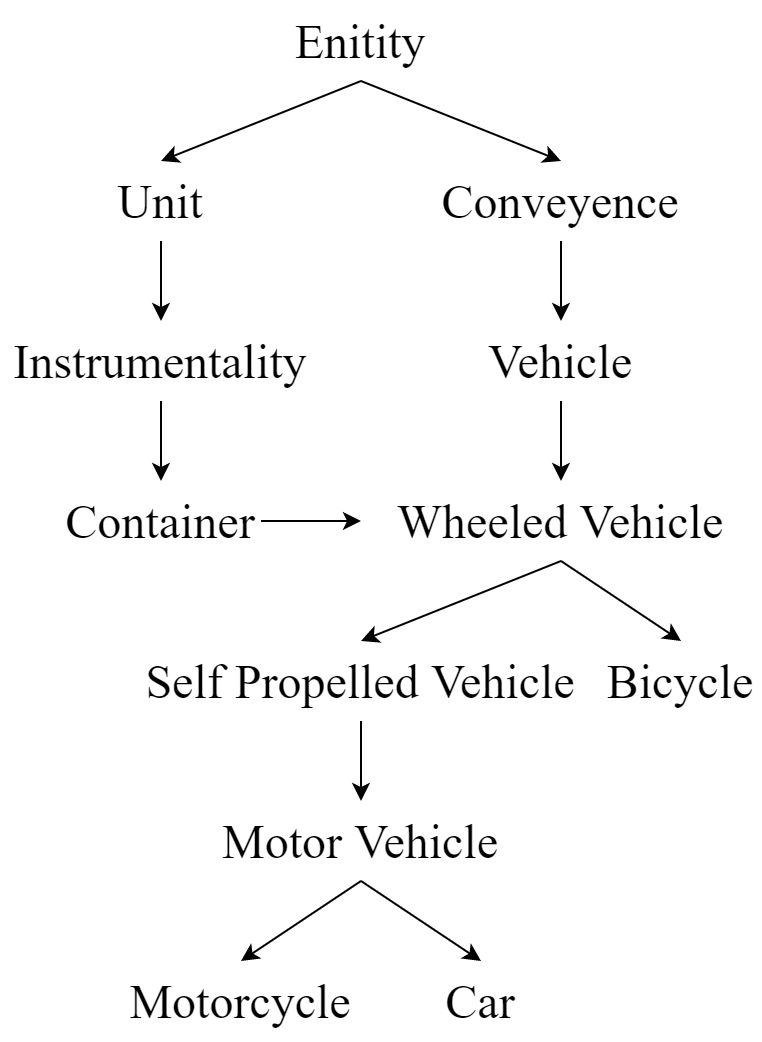
\includegraphics[width=250px]{WordNet.png}
  \caption[Cosine Similarity Alignment]{This figure shows the hierarchical structure from WordNet.}
  \label{fig:wordnet}
\end{figure}

% \subsection{Tongyici Cilin}
% 同義詞詞林由 Mei et al. (1983) 完成,收錄了五萬三千多個詞。因年代久遠,許多用詞與現在已經差異很大,後來由 HIT 修編為同義詞詞林擴增版,擴增為七萬多個詞,並放在由 HIT 所建立的 Language Technology Platform Cloud 上供大家下載與研究。
\paragraph{}
Tongyici Cilin (or Chinese Synonym Forest) wrote by Mei et al. (1983)\cite{mei1983hit}, there are 53k words collected. There are many terms changed these day, so the Harbin Institute of Technology Information Retrieval Lab (HIT IR Lab)\footnote{http://ir.hit.edu.cn/} extended Tongyici Cilin to collected over 70k words and removed both the old words and the uncommon words. The Tongyici Cilin [Extended] is provided on the Language Technology Platform Cloud\footnote{https://www.ltp-cloud.com/} build by HIT for peoples to download and research.

\paragraph{}
The original Tongyici Cilin provides three levels of encoding, the level 1 using an upper letter, the level 2 using a lower letter, and a two-digit number for the level 3. There are additional level 4 and level 5 in HIT Extended, an upper letter for the level 4, and a two-digit number for the level 5. There is a category symbol follow by each encoding, ``='' represents synonym words, ``\#'' represents similar words, and ``@'' represents independent words.

\begin{table}[H]
  \centering
  \begin{tabular}{ll}
  Encoding & Words \\
  \texttt{Ba01A02=} & 物質\ 質\ 素 \\
  \texttt{Cb02A01=} & 東南西北\ 四方 \\
  \texttt{Ba01A03@} & 萬物 \\
  \texttt{Cb06E09@} & 民間 \\
  \texttt{Ba01B08\#} & 固體\ 液體\ 氣體\ 流體\ 半流體 \\
  \texttt{Ba01B10\#} & 導體\ 半導體\ 超導體
  \end{tabular}
  \caption*{Samples of Tongyici Cilin {[}Extended{]}}
  \label{table:tc_sample}
\end{table}

\begin{table}[H]
  \centering
  \begin{tabular}{|l|C{1cm}|C{1cm}|C{1cm}|C{1cm}|C{1cm}|C{1cm}|C{1cm}|C{1cm}|}
  \hline
  Digits & 1 & 2 & 3 & 4 & 5 & 6 & 7 & 8 \\ \hline
  Example & D & a & 1 & 5 & B & 0 & 2 & \textbackslash{}=\#@ \\ \hline
  Level & Lv1 & Lv2 & \multicolumn{2}{c|}{Lv3} & Lv4 & \multicolumn{2}{c|}{Lv5} &  \\ \hline
  \end{tabular}
  \caption{Tongyici Cilin {[}Extended{]} encoding table.}
  \label{table:tc_encoding}
\end{table}

\paragraph{}
Using WordNet through NLTK (Natural Language Toolkit)\cite{nltk} to calculate the WUP similarity\cite{wu-palmer-1994-verb}.

\begin{equation}
  wup(s_1,s_2)=\frac{2\times depth(lcs)}{depth(s_1)+depth(s_2)}
\end{equation}

\paragraph{}
% 我們可以使用 NLTK 來找到 LCS,並透過節點的深度計算出兩個 synsets 的相似度。因為每個內容詞可能有不只一個 synsets,所以我們定義兩個內容詞 c1 和 c2 的 wup 相似度如下
We can find the LCS (least common subsumer) with NLTK and calculate the depth of synsets to get WUP similarity. Because each content word may has more than one synset, we defined WUP similarity of content words $c_1$ and $c_2$ as following.

\begin{equation}
  sim(c_1,c_2)=\max\limits_{\substack{s_1\in synsets(c_1) \\ s_2\in synsets(c_2)}} wup(s_1,s_2)
\end{equation}

\paragraph{}
Using the Tongyici Cilin to calculate the lv5 Similarity.

\begin{equation}
  lv5(C_1,C_2)=\frac{1}{|C_1|}\sum\limits_{c_1\in C_1}\max\limits_{c_2\in C_2} sim(c_1,c_2)
\end{equation}

\paragraph{}
% 因為中文的部份缺少完善的 WordNet 資源,而英文的部份則是缺少同義詞詞林的資源,所以這部份會透過 Cosine Similarity 來取代。
Because lack of a proper WordNet resource in Chinese and synonym forest in English, it is unable to calculate WUP similarity in Chinese and lv5 similarity in English. They will be replaced with the cosine similarity.

\begin{equation}
  similarity=\frac{A\cdot B}{||A||\ ||B||}=\frac{\sum\limits^{n}_{i=1}A_iB_i}{\sqrt{\sum\limits^{n}_{i=1}A^2_i}\sqrt{\sum\limits^{n}_{i=1}B^2_i}}
\end{equation}

\paragraph{}
The semantic features in English is listed below:

\begin{enumerate}
  \item[17.] average of cosine similarity $(t_1)$
  \item[18.] average of cosine similarity $(t_2)$
  \item[19.] average of WUP similarity $(t_1)$
  \item[20.] average of WUP similarity $(t_2)$
\end{enumerate}

\paragraph{}
The semantic features in Chinese is listed below:

\begin{enumerate}
  \item[17.] average of cosine similarity $(t_1)$
  \item[18.] average of cosine similarity $(t_2)$
  \item[19.] average of lv5 similarity $(t_1)$
  \item[20.] average of lv5 similarity $(t_2)$
\end{enumerate}

\subsubsection{Sentence Embedding}
\paragraph{}
% 因為句對間的蘊含關係有時並不需要用到整句話的資訊,只需要部份資訊,因此 Sentence Embedding 這種呈現 sentence features 的方法就是個不錯的選擇。Sentence Embedding 是由 Word Embedding 的向量計算而來,而關於 Word Embedding 的詳細敘述,請參考 Word Embedding 章節。在本論文中,我們選擇使用單純的總和平均做為計算 Sentence Embedding 的方法。
The entailment relation between the premise and the hypothesis sometimes does not need the information of the whole sentence, the partial information of the sentence is enough, so sentence embedding is an efficient method to represent the partial information of the sentence features. The sentence embedding is calculated from word embedding, the detailed discussion of word embedding please refer to the section \ref{section:word_embedding}. In this thesis, we simply choose the arithmetic mean as the calculation of sentence embedding.

\subsection{Word-based Sequence Input} \label{section:word_embedding}
\subsubsection{Raw Text Input}
\paragraph{}
% 在自然語言領域裡使用深度學習時,經常使用將每個字詞表達成一組向量的方法,將這組詞向量根據句子做排列而得到的詞向量序列做為神經網路的輸入層特徵。而在 RTE 任務裡,我們將 Premise 和 Hypothesis 串接起來,並在中間加入一個特殊 Token <SEP> 做為區隔。用來表達詞向量的方法有很多種,我們將在接下來的章節介紹這些語言模型。
When using deep learning in the field of natural language process, it is common to represent each word as a vector and combined it as a sequence of word vectors according to the order of the sentence, this word-based sequence will be the input features of the neural network. In the recognizing textual entailment task, we concatenated the sequence of word vectors of the premise and the hypothesis, a special token ``\texttt{[SEP]}'' will be put in the middle as the separator. There are many methods to represent the word embedding, we will introduce them in the following sections.

\subsubsubsection{Self-Trained Word Embedding}
\paragraph{}
% 與 Pre-trained Word Embedding 不同,Self-trained Embedding 通常做為神經網路的其中一個 Layer,並透過神經網路的梯度傳導機制不斷調整每個字詞的向量,根據任務的方向去學習適當的權重。Pre-trained Word Embedding 通常只會適合 Pretraining 時所使用的文本領域,若是 Pretraining 時的文本領域不夠廣泛或過於特殊,可能會對實驗效能有不好的影響。但因為 Self-trained Word Embedding 可以根據任務文本去進行彈性調整,所以在特定領域可能會有更好的表現,但也有可能因為資料數量不足的關係而使效能有所限制。
Different from the pre-trained word embedding, self-trained embedding usually use as a layer of a neural network and adjust each word vector through the backpropagation mechanism of the neural network. To the pre-trained word embedding, the suitable task is limited by the pre-training corpus. If the pre-training corpus is not common enough, it might have a bad influence on the experiments. The self-trained word embedding can do flexible adjustment according to the domain of the task text, therefore the performance may be better in a certain domain, but also may be limited by the data size of the training dataset.

\subsubsubsection{fastText}
\paragraph{}
fastText\cite{bojanowski2016enriching} is a library for efficient text classification and representation learning created by Facebook's AI Research (FAIR) lab. This library allows us to create word embedding with unsupervised learning algorithms, like skip-gram and continuous bag-of-word (CBOW). With this library, we train a word representation from Traditional Chinese Wikipedia, both in the version of skip-gram and CBOW, the embedding size is 250.

\subsubsubsection{Google NNLM}
\paragraph{}
Google NNLM is provided by TensorFlow Hub\footnote{https://www.tensorflow.org/hub} which has many different language models that already be trained by a large corpus. We use the Chinese version of NNLM that trained on Simplified Chinese Google News 100B corpus and publish by Google\footnote{https://tfhub.dev/google/tf2-preview/nnlm-zh-dim128/1}. In order to fit the Traditional Chinese dataset, we convert the dictionary of the Google NNLM from Simplified Chinese into Traditional Chinese.
% BERT Language Model

\subsubsection{Word-Alignment Groups} \label{section:csa}
% 指的是 CSA 但要講得比現在版本更清楚、要想像

\paragraph{}
We propose a new method to do alignment by calculating the cosine similarity between words of two sentences and set a ``similarity threshold'' to define if the two words will be aligned. The similarity threshold is variable and we will observe the impact of the change of the value of the similarity threshold.

\paragraph{}
% 首先先計算兩句話的每個詞之間的 Cosine Similarity 建立一個 Similarity Table,然後從表中挑出相似數值最高的兩個詞,將 premise 的詞放入 list1 並將 hypothesis 的詞放入 list2,然後將這兩個詞從表中刪去,再繼續往下挑相似數值最高的兩個詞,直到該相似數值小於 Similarity Threshold 為止。接下來把 premise 剩下的詞一個一個放入 list1,每放一個詞到 list1 裡面,就在 list2 裡面放一個零,hypothesis 剩下的詞也是一樣的操作。最後將 list2 的值減去 list1 獲得最後的 CSA Features。
First, we calculated the cosine similarity of each word of two sentences to build a similarity table, then picked up the word pair with the highest value of similarity, and put the word vector of the word from the premise sentence into $list_1$ and put the one from the hypothesis sentence into $list_2$ and remove the two words from the similarity table. Repeat this step until the highest value of the similarity is lower than the similarity threshold. Next, we put the word vectors of the left words of the premise sentence into $list_1$ one by one, every time we put a word vector into $list_1$, put a zero vector into $list_2$, and do the same operation to the left words of the hypothesis sentence, so the two lists will remain the same size. After all, we use $list_2$ to minus $list_1$ to obtain the final ``CSA Features''.

\begin{figure}[!ht]
  \centering
  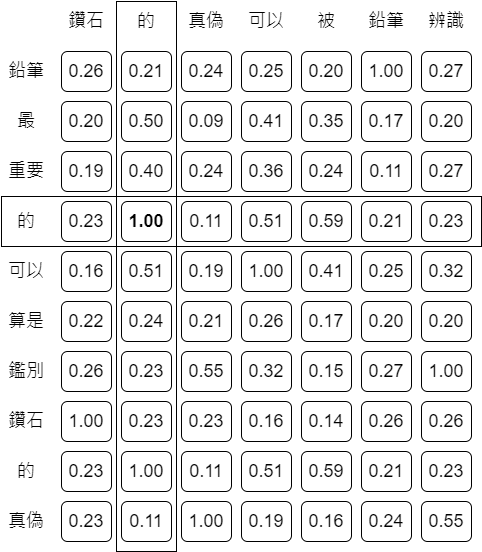
\includegraphics[width=175px]{CSA.png}
  % 此圖顯示兩句話裡每個字之間的 Cosine Similarity,每個字將會根據這個 Cosine Similarity Table 進行 Alignment
  \caption[Cosine Similarity Alignment]{This figure shows the calculation of cosine similarity between words of sentence pair, the words will be aligned by this cosine similarity table.}
  \label{fig:csa}
\end{figure}

\subsection{Classifier}

\subsubsection{Neural Network}
\paragraph{}
% 神經網路的蓬勃發展使機器學習在各領域上都獲得了不小幅度的進展,
% Dense Neural Network, Recurrent Neural Network (LSTM, GRU), Attention Mechanism, Transformers
% Simple DNN 模型是只使用了一層 Dense Layer 的模型,透過 Tensorflow 套件建立而成。這個模型架構設計很單純,只用來接收 ML Features。
A simple DNN model is a neural network only contains one dense layer as a hidden layer, building by Tensorflow API. This model architecture is pretty simple, only use to receive machine learning features.

\subsubsection{RNN-Attention Model}
\paragraph{}
% RNN-Attention 模型是數種由不同數量與順序的 RNN Layers 與 Attention Layers 組合而成的模型
The RNN-Attention Model (RA Model) is a combination of several different numbers and orders of RNN layers and attention layers.

The attention mechanism is described in Vaswani et al. (2017)

\subsubsection{BERT}
\paragraph{}
The structure of transformer\cite{vaswani2017attention} has been described in Vaswani et al., 2017, they use multi-head attention to build the encoder-decoder model, which uses to solve the machine translation tasks. On the other hand, BERT\cite{devlin2018bert} (Devlin et al., 2019) also used the transformer architecture to achieve excellent performance on several natural language processing tasks, including MNLI, QNLI, and RTE which are contained in GLUE benchmark. The source code of BERT are available on GitHub\footnote{https://github.com/google-research/bert} and it can be easily called using HuggingFace Transformers API\cite{wolf-etal-2020-transformers}.

\paragraph{}
There are many different models from the official GitHub repository, like the \texttt{bert-base-cased} model is pre-trained by cased English corpus and the \texttt{bert-base-chinese} model is pre-trained by both Traditional Chinese and Simplified Chinese corpus. Besides these language-specific models, the most important model is the cross-lingual model like the \texttt{bert-base-multilingual-cased} model, which allows us to train and fine-tune with different languages in one model easily.

\section{Training Data Augmentation} \label{section:pseudo}
\subsection{Adding Other NLI Datasets}
% 近年來與深度學習相關的研究顯示資料量是影響系統效能相當大的關鍵之一,當資料量超過萬筆之後,系統效能會有顯著的提昇。然而無論是 RITE2 或 RITE-VAL,僅一千多筆的資料規模在展現深度學習的效能上顯得十分有限。因此我們將其他 NLI 資料集加入訓練資料以增加資料規模,進一步提昇模型的效能。在這部份,資料集改造的方法有分兩種:第一種是直接將其他資料集與 RITE 的訓練資料做混合做為新的訓練資料,第二種則是先用其他資料集做預訓練,再使用 RITE 的訓練資料進行 Fine-tune。
\paragraph{}
The research of deep learning in recent years has shown that the scale of data size has a huge impact on the performance of the system, there will be a significant improvement when the amount of data comes over ten thousand. However, no matter on RITE2 or RITE-VAL, only over a thousand amounts of data is not enough to show off the ability of deep learning. Therefore we augmented the training data with the other NLI datasets to increase the scale of the data size and further improve the performance of the model. We have two methods in the data augmentation, the first is to mix the original training set of RITE with the other datasets as a new training set, the second is using the other datasets to pre-train the model and fine-tune with the training set of RITE.

% 基本上在任何實驗都可以使用 CNLI 與 OCNLI 等與 RITE 相同語言的資料集進行相同的訓練手法,而在 BERT 的跨語言模型上可以進一步使用不同語言的資料集來做訓練,例如 MNLI。
\paragraph{}
Basically, We do the same training trick on any experiments by using the datasets that have the same language with RITE, such as CNLI and OCNLI, and on the multi-lingual model of BERT, we can even use the datasets that have the different language to improve our system.

\subsection{Pseudo Training Data}
% 我們嘗試使用大量的虛擬資料來改進模型的效能,虛擬資料的產生方式則有規則式改寫與 GPT2 模型生成兩種。這兩種方法會對四個標籤都產生等量的資料,並根據 MNLI 的資料量,各產生 400k 組句對。在接下來的章節會介紹產生虛擬資料的細節。
\paragraph{}
We try to use large-scale pseudo dataset to improve the performance of the model, and the generating methods of the pseudo training data are rule-based rewriting and GPT2 model generation. Both of the methods will generate an equal amount of data for the four labels. According to the data size of the MNLI dataset, each of the methods will generate 400k sentence pairs. We will introduce the details of the pseudo training data generation in the following sections.


\subsubsection{CIRB}
% CIRB, Synonym Dictionary, Antonym Dictionary, Negative Words
% 首先我們先介紹產生虛擬訓練資料會需要用到的資源。因為產生虛擬資料的方法基本上是透過改寫句子得來的,而改寫規則未必能夠適用於任何句子上,因此我們需要有足夠大量的文章才能確保生成的句子數量是充足的。CIRB (Chinese Information Retrieval Benchmark) 是一份來自 NTCIR 2 資訊檢索子任務的測試集,蒐集了 1998 年到 2005 年間五家線上新聞媒體的新聞文章資料,總共 280 萬篇文章,每篇文章的長度平均為 560 個字,包含的領域廣泛分佈於政治、財經、體育、娛樂、科技、國際等。且 RITE 資料集本身也有一些句子是來自於新聞文章,所以我們認為 CIRB 是一個相當合適的資料集。
\paragraph{}
First, we will introduce the resources used in the generation of pseudo training data. Most of the generated data come from the modification of sentences and the rewriting rules may not be applied to any sentences, so we need to ensure the number of the articles is enough to generate sufficient sentences. The CIRB (Chinese Information Retrieval Benchmark)\cite{chen2001cirb} dataset is a test collection of the Chinese information retrieval tasks of NTCIR 2 which collected the news articles released from the websites of Chinatimes\footnote{https://www.chinatimes.com/}, Chinatimes Commercial\footnote{https://ctee.com.tw/}, Chinatimes Express, Central Daily News, and China Daily News during 1998 to 2005. There are in total 2.8 million articles with an average length of 560 characters. The domains covered are widely distributed in politics, finance, sports, entertainment, technology, and international. Besides, the part of sentences in the RITE dataset also comes from the news article, so we think the CIRB collection is a suitable corpus for our purpose.

\subsubsection{Synonym and Antonym}
% 在產生過程中,我們會需要用到同義詞辭典與反義詞辭典。透過 HIT 我們可以很輕易的建立起同義詞辭典,而反義詞辭典則需要透過英文 WordNet 與中文 WordNet 來建立。
\paragraph{}
We need to use the synonym dictionary and the antonym dictionary to generate the pseudo training data. It is easy to build the synonym dictionary using the Tongyici Cilin by the well-organized synonym encoding.
% 使用 Sinica BOW (Bilingual Ontological Wordnet)\cite{huang2004sinica}

\subsubsection{Rule-Based}
% 在規則式的部份,我們首先使用替換法的方式來產生句對,替換的對象包含同義詞與反義詞。我們從 Corpus 中隨機挑選出一個由二到三個短句所構成的句子,並從句中尋找一個存在於同義詞辭典或反義詞辭典的詞來進行替換。同義詞辭典來自於同義詞詞林,而反義詞辭典則來自於中英 WordNet 的對應。因為可替換的詞可能不只一個,所以會優先使用字數相近的詞。接下來,我們嘗試在句中隨機加入否定詞。我們先計算了整個 Corpus 裡面否定詞詞性的 N-Gram 機率,再從隨機挑選的句子中尋找詞性 N-Gram 機率較高的位置插入否定詞。上述的做法都只會替換或插入一個詞。以同義詞替換而產生的句對被標記為 B,以反義詞替換而產生的句對被標記為 C,以隨機插入否定詞而產生的句對被標記為 C。
\paragraph{}
In the rule-based method, we first use the substitution method to generate sentence pairs, and the targets of substitution include synonyms and antonyms. We randomly select a long sentence consisting of 2 to 3 short sentences from the corpus and search for a word from the existing sentences in the antonym or synonym dictionary to replace it. The synonym dictionary comes from HIT, and the antonym dictionary comes from the mapping of English WordNet and Chinese WordNet. Because there will be more than one word that can be replaced in a sentence, a similar number of characters will be used. Next, we try to add negative words into sentences randomly. We first calculate the n-gram probability of the sentences including negative words and insert a negative word into the position with the highest probability. The methods above will only replace or insert one word, the augmented sentence will be seen as the hypothesis and combined with the original sentence as new sentence pair. The sentence pairs generated by synonym substitution will be marked as ``bi-directional''. The sentence pairs generated by antonym substitution will be marked as ``contradiction''. The sentence pairs generated by negative word insertion will be marked as ``contradiction''.

% 為了更進一步擴展我們的資料集,我們將產生出來的句子以逗號為邊界,將句子分割成數個短句,並將這些短句與原本的句子重新組成新的句對。若是該短句沒有被改造過,則新的句對被標記為 F;若是該短句被改造過且原本被標記為 C,則新的句對同樣被標記為 C;若是該短句被改造過且原本被標記為 B,則新的句對會被標記為 F。
\paragraph{}
To further expand our dataset, we split the sentence into several short sentences according to the comma and combined each of these short sentences with the original sentences as new sentence pairs. If the new sentence has not been modified, the new sentence pair will be marked as ``forward entailment''. If the new sentence has been modified and originally marked as ``contradiction'', the new sentence pair will also be marked as ``contradiction''. If the new sentence has been modified and originally marked as ``bi-directional'', the new sentence will be marked as ``forward entailment''.

% 最後,我們使用兩種單純的方法來產生 I 的資料。第一種是從 Corpus 裡面隨機挑選兩句組成一個句對;第二種是從 Corpus 裡面挑選一個長句,並將其斷成前後兩句,由這兩句話組成一個句對。
\paragraph{}
Finally, we use two simple ways to generate ``independence'' sentence pairs. The first is to randomly pick two sentences from corpus as a sentence pair, the second is to randomly pick a long sentence from corpus, and split it into two sentence as new sentence pair.

% Synonmy
% 失控所致或營造而成,差異極大
% 失控所致或營造而成,反差極大
% Split 1
% 失控所致或營造而成,差異極大
% 失控所致或營造而成
% Split 2
% 失控所致或營造而成,差異極大
% 反差極大

% Antonym
% 即日起上市,可預約宅配
% 即日起上市,不許預約宅配
% Split 1
% 即日起上市,可預約宅配
% 即日起上市
% Split 2
% 即日起上市,可預約宅配
% 不許預約宅配

% Negative
% 相較之下,台灣藝術家以公共藝術文化輸出的案例卻未聽聞
% 相較之下,台灣藝術家以非公共藝術文化輸出的案例卻未聽聞
% Split 1
% 相較之下,台灣藝術家以公共藝術文化輸出的案例卻未聽聞
% 相較之下
% Split 2
% 相較之下,台灣藝術家以公共藝術文化輸出的案例卻未聽聞
% 台灣藝術家以非公共藝術文化輸出的案例卻未聽聞

\begin{table}[ht!]
  \centering
  \begin{tabular}{|l|l|c|}
    \hline
    \multicolumn{1}{|c|}{Method} & \multicolumn{1}{c|}{Sentence Pair} & Label \\ \hline
    \multirow{2}{*}{Synonym} & 失控所致或營造而成,差異極大 & \multirow{2}{*}{B} \\ \cline{2-2}
    & 失控所致或營造而成,反差極大 &  \\ \hline
    \multirow{2}{*}{Synonym \& Split (1)} & 失控所致或營造而成,差異極大 & \multirow{2}{*}{F} \\ \cline{2-2}
    & 失控所致或營造而成 &  \\ \hline
    \multirow{2}{*}{Synonym \& Split (2)} & 失控所致或營造而成,差異極大 & \multirow{2}{*}{F} \\ \cline{2-2}
    & 反差極大 &  \\ \hline
    \multirow{2}{*}{Antonym} & 即日起上市,可預約宅配 & \multirow{2}{*}{C} \\ \cline{2-2}
    & 即日起上市,不許預約宅配 &  \\ \hline
    \multirow{2}{*}{Antonym \& Split (1)} & 即日起上市,可預約宅配 & \multirow{2}{*}{F} \\ \cline{2-2}
    & 即日起上市 &  \\ \hline
    \multirow{2}{*}{Antonym \& Split (2)} & 即日起上市,可預約宅配 & \multirow{2}{*}{C} \\ \cline{2-2}
    & 不許預約宅配 &  \\ \hline
    \multirow{2}{*}{Negative} & 相較之下,台灣藝術家以公共藝術文化輸出的案例卻未聽聞 & \multirow{2}{*}{C} \\ \cline{2-2}
    & 相較之下,台灣藝術家以非公共藝術文化輸出的案例卻未聽聞 &  \\ \hline
    \multirow{2}{*}{Negative \& Split} & 相較之下,台灣藝術家以公共藝術文化輸出的案例卻未聽聞 & \multirow{2}{*}{C} \\ \cline{2-2}
    & 台灣藝術家以非公共藝術文化輸出的案例卻未聽聞 &  \\ \hline
  \end{tabular}
  \caption{Example of sentence pair generated by rule-based methods.}
  \label{example:sim_nli_rule_based}
\end{table}

\subsubsection{GPT2 Generation}
% GPT2 \cite 是由 OpenAI 所開發的一個自然語言產生模型,在機器翻譯、問答、總結和文本產生都有相當出色的表現。而透過 GPT2 模型產生虛擬資料的這個實驗,我們參考了 _ 論文中的做法,從 Corpus 中隨機挑選句子,並將非內容詞去除,只留下內容詞做為「head seed」,然後將完整的句子拼接在 head seed 後面,目的是訓練 GPT2 模型在餵入這些內容詞後,可以產生完整的句子。在適當的訓練下,對 GPT2 模型餵入相同的內容詞做為 head seed 可以產生不同但相似的句子。
\paragraph{}
GPT2\cite{radford2019language} is a natural language generation model created by OpenAI, it has an excellent performance in machine translation, question answering, summarization, and text generation. The GPT2 generation method of the simulation dataset is based on Hegde et al. (2020)\cite{hegde2020unsupervised}. We randomly picked sentences from the corpus and removed the non-content word, only remain the content words as the seeds of GPT2, then we concatenated the original sentence after the seeds. We use special tokens to surround the seeds, so the model can distinguish the seeds and the sentence. Our purpose is to train the GPT2 model can generate a complete sentence including the words of the seeds. With proper training, the GPT2 model can generate different but similar sentences from the same seeds.

% 我們保留訓練資料中的原句做為 Premise,並使用相同的 head seed 產生一個句子做為 Hypothesis ,這樣獲得的句對可以標記為 B。接下來,我們透過更換 head seed 的內容詞來產生其他不同標記的句對。從 head seed 中隨機挑選兩個詞並互換位置,這樣產生的句對為 B。將 head seed 中的部份內容詞去除,這樣產生的句對為 F。從 head seed 中隨機挑選一個內容詞變成反義詞,這樣產生的句對為 C。隨機插入一個否定詞在 head seed 裡面,產生出來的句對為 C。只保留一個 head seed 的內容詞,並隨機放入其他內容詞,產生出來的句對為 I。
\paragraph{}
We keep the original sentence of the training example as the premise sentence and use the same seeds from the training example to generate a new sentence as the hypothesis sentence. These sentence pairs will be marked as ``bi-directional''. Next, we will generate sentences for different labels by changing the word of seeds. Randomly picked one word and replace it with synonym, the generated sentence pairs will be marked as ``bi-directional''. Randomly picked two words of seeds and exchanged their position, the generated sentence pairs will be marked as ``bi-directional''. Randomly remove 1~3 words of seeds, the generated sentence pairs will be marked as ``forward entailment''. Randomly picked one content word and replace it with an antonym, the generated sentence pairs will be marked as ``contradiction''. Randomly insert a negative word in seeds, the generated sentence pairs will be marked as ``contradiction''. At last, only remain one content word of seeds and put 3~10 random words within, the generated sentence pairs will be marked as ``independence''.

\begin{table}
  \centering
  \begin{tabular}{|l|l|l|c|}
  \hline
  \multicolumn{1}{|c|}{Method} & \multicolumn{1}{c|}{Seed} & \multicolumn{1}{c|}{Generated Sentence} & Label \\ \hline
  Original & {[}CLS{]} 無 理性 能力 {[}SEP{]} & 以致無理性思考的能力。 & - \\ \hline
  Same & {[}CLS{]} 無 理性 能力 {[}SEP{]} & 是極端無理性的能力。 & B \\ \hline
  Exchange & {[}CLS{]} 理性 無 能力 {[}SEP{]} & 只有理性和無能力。 & B \\ \hline
  Synonym & {[}CLS{]} 非 理性 能力 {[}SEP{]} & 也是非理性能力的一種。 & B \\ \hline
  Remove & {[}CLS{]} 無 能力 {[}SEP{]} & 還是無能力了! & F \\ \hline
  Antonym & {[}CLS{]} 所有 理性 無資格 {[}SEP{]} & 或是所有理性的人都無資格。 & C \\ \hline
  Negative & {[}CLS{]} 非 理性 無 能力 {[}SEP{]} & 一般是非理性、無能力 & C \\ \hline
  Random & {[}CLS{]} 出發 能力 表達 清楚 {[}SEP{]} & 出發雖有能力,但卻表達不清楚。 & I \\ \hline
  \end{tabular}
  \caption{Example of sentence generated by GPT2.}
  \label{example:gpt2_pseudo}
\end{table}

% 我們使用 CIRB 做為 Corpus,並根據四個標籤平均生成資料集,每個標籤下的每一種方法也同樣生成平均數量的資料。規則式與 GPT2 根據 MNLI 的資料集規模,各自生成四十萬組句對,總共生成八十萬組句對。
\paragraph{}
We generate the dataset equally according to the four labels, each generation method also generates an equal number of data under each label. Both rule-based and GPT2 will generate 400k sentence pairs that similar to the data size scale of the MNLI dataset, 800k sentence pairs are generated totally.

\begin{table}
  \centering
  \begin{tabular}{|l|l|c|r|c|}
  \hline
  \multicolumn{1}{|c|}{System} & \multicolumn{1}{c|}{Method} & Label & \multicolumn{1}{c|}{Number} & Total \\ \hline
  \multirow{10}{*}{Rule-Based} & Synonym & B & 100k & \multirow{10}{*}{400k} \\ \cline{2-4}
   & Antonym & C & 25k &  \\ \cline{2-4}
   & Negative Word & C & 25k &  \\ \cline{2-4}
   & Antonym and Split (1) & C & 25k &  \\ \cline{2-4}
   & Negative Word and Split (1) & C & 25k &  \\ \cline{2-4}
   & Synonym and Split & F & 33k &  \\ \cline{2-4}
   & Antonym and Split (2) & F & 33k &  \\ \cline{2-4}
   & Negative Word and Split (2) & F & 33k &  \\ \cline{2-4}
   & Radom Pick & I & 50k &  \\ \cline{2-4}
   & Random Split & I & 50k &  \\ \hline
  \multirow{7}{*}{GPT2} & Same Seed & B & 33k & \multirow{7}{*}{400k} \\ \cline{2-4}
   & Synonym & B & 33k &  \\ \cline{2-4}
   & Exchange Position & B & 33k &  \\ \cline{2-4}
   & Random Remove & F & 100k &  \\ \cline{2-4}
   & Antonym & C & 50k &  \\ \cline{2-4}
   & Negative Word & C & 50k &  \\ \cline{2-4}
   & Remain One & I & 100k &  \\ \hline
  \end{tabular}
  \caption{The pseudo training data distribution.}
  \label{table:pseudo_training_data_dist}
\end{table}

\section{Experiments} \label{section:experiments}
\subsection{Datasets and Evaluation Metrics}
\paragraph{}
% 根據 NTCIR 主辦單位提供的正式評估公式來計算 macroF1
According to the formal evaluation formula provided by NTCIR:

\begin{equation}
  macroF1=\frac{1}{|C|}\sum_{c\in C}F1_c
\end{equation}

\paragraph{}
$C$ is all categories, and $c$ is one of the categories. Because $macroF1$ is the average of F1-Score to each category, it won't be affected by a category that has a large number. The experiments of the BFCI task will use this evaluation formula.

\paragraph{}
F-measure also called F1-score, is a measure that is calculated from precision and recall. It is usually used in the information retrieval field to compare the different systems. F1-score, precision, and recall are defined as follows.

\begin{equation}
  F1=\frac{2\times Precision\times Recall}{Precision+Recall}
\end{equation}

\begin{equation}
  Precision=\frac{N_{correct}}{N_{predicted}}
\end{equation}

\begin{equation}
  Recall=\frac{N_{correct}}{N_{target}}
\end{equation}

\paragraph{}
% 在 RITE 的實驗中,我們對 Training Set 進行 10-Fold Cross-validation,並計算這十個 Fold 的 Micro F1-Score 做為評估結果之一。而測試集的部份則以 10-Fold 產生出來的 10 個權重各評估一次並取平均做為 Test F1-Score。
In the experiments of RITE, we do the 10-fold cross-validation to the training set and calculate the micro F1-score as one of the evaluation results. We evaluate the test set by each model weight of the ten folds, then take the average as test F1-score.

\paragraph{}
To compare the experiments of the ECN tasks with the other systems, we use accuracy as the evaluation formula of the ECN tasks.

\paragraph{}
To understand the impact of the characters of the Traditional and the Simplified, we use OpenCC\footnote{https://github.com/BYVoid/OpenCC} which available as a python package to convert CNLI and OCNLI into CNLI-TW and OCNLI-TW.

\subsection{Machine Learning Feature Experiments}
% 首先我們重製了 Liu 等人的 SVM 實驗,並與 SimpleDNN 做比較。在 Scikit-Learn 套件中提供了四個 Kernel: RBF, Linear, Sigmoid, and Poly,所以我們先比較了不同的 SVM Kernel。
% 在 Liu 等人的實驗中,分別將 Lexical (lex), Syntactic (syn), Word Similarity (wn), 與 Synonym Forest (cl) 各自去除,來測試哪個特徵對實驗結果的影響較大。而在 SimpleDNN 的實驗中,我們也做了相同的步驟。
% 接下來,我們嘗試用基本的 RNN Model 來進行實驗。RNN 的部份測試了 LSTM 與 GRU 以及各自加上 Attention 的效果,在 Word Embedding 的部份則測試了 Self-trained, fastText CBOW, fastText Skip-gram, 與 GoogleNNLM。其結果如表:(待補)
% (st/ftCBOW/ftSG/g x LSTM/GRU x with/without Attention)
% 在這個實驗的基礎上,我們將 ML Features 結合到 RNN Model 裡面。我們將 RNN Encoder 的 Output 與 ML Features 做 Concatenate 後再進行分類,其結果如表(待補)
% 而在本論文中,我們提出了 CSA 方法,並將 CSA 特徵放入 RNN Model,也分別測試了與 ML Features 或 Word Embedding 做結合的實驗,其結果如表:(待補)
\paragraph{}
To cross-compare the performance of datasets, we first extended the RITE-VAL with reversed labels to generate RITE-VAL-REV and mixed RITE2 with RITE-VAL-REV to generate RITE-VAL-REV-2. So we have RITE2, RITE-VAL, RITE-VAL-REV, and RITE-VAL-REV-2 to be used as the training sets. The test sets of RITE2 and RITE-VAL will be marked as RITE2-TEST and RITE-VAL-TEST.

\paragraph{}
% SVM 的實驗結果:Kernel Comparison
The Scikit-Learn package provides four types of kernels of SVM: RBF, Linear, Sigmoid, and Poly. We want to figure out which kernel is the most suitable, so we use the ML features mentioned in \ref{section:ml_features} to compare the performance of kernels of SVM. From table \ref{svm_kernel} we can see that both in RITE-VAL and RITE2, RBF kernel is the most suitable kernel of SVM, so we use RBF kernel as the default kernel in the following experiments.

\begin{table}[H]
  \centering
  \begin{tabular}{|L{1.5cm}|R{1.5cm}|R{1.5cm}|R{1.5cm}|R{1.5cm}|}
  \hline
  \multicolumn{5}{|c|}{SVM Kernels Comparison} \\ \hline
  \multicolumn{1}{|c|}{Kernel} & \multicolumn{1}{c|}{RBF} & \multicolumn{1}{c|}{Linear} & \multicolumn{1}{c|}{Sigmoid} & \multicolumn{1}{c|}{Poly} \\ \hline
  \multicolumn{5}{|c|}{Validation Target: RITE-VAL} \\ \hline
  all & 0.4011 & 0.3538 & 0.2696 & 0.3495 \\ \hline
  all - lex & 0.4047 & 0.3449 & 0.3434 & 0.3510 \\ \hline
  all - syn & 0.4045 & 0.3567 & 0.2701 & 0.3547 \\ \hline
  all - wn & \textbf{0.4122} & 0.3560 & 0.3090 & 0.3539 \\ \hline
  all - cl & 0.3978 & 0.3539 & 0.3043 & 0.3445 \\ \hline
  \multicolumn{5}{|c|}{Validation Target: RITE2} \\ \hline
  all & 0.5177 & 0.4872 & 0.3126 & 0.4949 \\ \hline
  all - lex & 0.4868 & 0.4555 & 0.3176 & 0.4712 \\ \hline
  all - syn & 0.4997 & 0.4923 & 0.2509 & 0.4741 \\ \hline
  all - wn & 0.4941 & 0.4766 & 0.3158 & 0.4902 \\ \hline
  all - cl & \textbf{0.5410} & 0.4871 & 0.3172 & 0.4928 \\ \hline
  \end{tabular}
  \caption{Results of SVM kernels comparison, the training data is RITE-VAL-REV-2. The performance is always better when the kernel is RBF.}
  \label{svm_kernel}
\end{table}

\paragraph{}
% 當 Training Source 是 RITE-VAL 的時候,Simple DNN 的效能可能不見得是最好的,我們認為這可能是因為 RITE-VAL 的資料規模相對較小,在資料規模不大的情況下 SVM 可以取得較好的效果。
We compare the performance of SVM and our simple DNN model. The hidden size of the hidden layer is 512, the optimizer is RMSprop, the learning rate is 5e-5, the batch size is 8, and training for 500 epochs. From table \ref{result:ml_original} we can see that the simple DNN has better performance in almost all cases, but when the training source is RITE-VAL, it seems that the simple DNN is not always the best. We think this may because of the relatively small-scale data size of RITE-VAL. When the data size is not large enough, the SVM will get better performance usually.

\begin{table}
  \centering
  \begin{tabular}{|l|R{2.5cm}|R{2.5cm}|R{2.5cm}|R{2.5cm}|}
  \hline
  Training Source & \multicolumn{2}{c|}{RITE-VAL} & \multicolumn{2}{c|}{RITE2} \\ \hline
  Classifier & \multicolumn{1}{c|}{SVM} & \multicolumn{1}{c|}{Simple DNN} & \multicolumn{1}{c|}{SVM} & \multicolumn{1}{c|}{Simple DNN} \\ \hline
  Validation Target & \multicolumn{4}{c|}{RITE-VAL} \\ \hline
  all & \textbf{0.3840} & 0.4107 & 0.4203 & \textbf{0.4665} \\ \hline
  all - lex & 0.3701 & \textbf{0.4146} & 0.3864 & 0.4479 \\ \hline
  all - syn & 0.3673 & 0.3726 & 0.4100 & 0.4355 \\ \hline
  all - wn & 0.3829 & 0.4134 & \textbf{0.4290} & 0.4641 \\ \hline
  all - cl & 0.3746 & 0.4098 & 0.4211 & 0.4653 \\ \hline
  Validation Target & \multicolumn{4}{c|}{RITE2} \\ \hline
  all & 0.3639 & 0.3655 & 0.5220 & 0.5936 \\ \hline
  all - lex & 0.3733 & 0.3590 & 0.4913 & 0.5654 \\ \hline
  all - syn & 0.3289 & 0.3457 & \textbf{0.5572} & 0.5516 \\ \hline
  all - wn & 0.3441 & 0.3598 & 0.4965 & 0.5820 \\ \hline
  all - cl & \textbf{0.3864} & \textbf{0.3752} & 0.5450 & \textbf{0.5954} \\ \hline
  Validation Target & \multicolumn{4}{c|}{RITE-VAL-TEST} \\ \hline
  all & \textbf{0.3522} & 0.3506 & 0.3427 & \textbf{0.3715} \\ \hline
  all - lex & 0.3428 & 0.3504 & 0.3537 & 0.3584 \\ \hline
  all - syn & 0.2839 & 0.2822 & 0.3375 & 0.3016 \\ \hline
  all - wn & 0.3500 & \textbf{0.3523} & 0.3435 & 0.3709 \\ \hline
  all - cl & 0.3294 & 0.3516 & \textbf{0.3598} & 0.3702 \\ \hline
  Validation Target & \multicolumn{4}{c|}{RITE2-TEST} \\ \hline
  all & 0.3413 & \textbf{0.3261} & 0.4527 & 0.4512 \\ \hline
  all - lex & 0.3319 & 0.3130 & 0.4119 & 0.4321 \\ \hline
  all - syn & 0.3455 & 0.3033 & 0.4386 & 0.4478 \\ \hline
  all - wn & 0.3273 & 0.3197 & 0.4566 & 0.4488 \\ \hline
  all - cl & \textbf{0.3559} & 0.3196 & \textbf{0.4616} & \textbf{0.4625} \\ \hline
  \end{tabular}
  \caption{Results of SVM and simple DNN comparison using original training data.}
  \label{result:ml_original}
\end{table}

\subsection{Sentence-Based Embedding Experiments}
% 在 Sentence-based embedding 的實驗中,我們將 Self-Trained Word Embedding, fastText CBOW, fastText Skip-gram 與 Google NNLM 等四種 NNLM 分別進行測試,sentence embedding 的算法為 word embedding 的平均,其結果如表。可見 fastText CBOW 的效果較好,我們認為這是 CBOW 的特性使得這個 NNLM 相當適合進行 Sentence Embedding 的實驗。
In the experiments of sentence-based embedding, we test the four types of word embedding: self-trained embedding, fastText CBOW, fastText skip-gram, and Google NNLM. The calculation of sentence embedding is the average of the word embedding of the sentence. The results are shown in table \ref{result:sent_emb_nnlm}, we can see that the performance of fastText CBOW is the best, it might because of the mechanism of the CBOW calculation to make this language model suitable with the experiments of sentence embedding.

\begin{table}[H]
  \centering
  \begin{tabular}{|l|r|r|r|r|}
  \hline
   & \multicolumn{2}{c|}{RITE-VAL} & \multicolumn{2}{c|}{RITE2} \\ \hline
   & \multicolumn{1}{c|}{Dev} & \multicolumn{1}{c|}{Test} & \multicolumn{1}{c|}{Dev} & \multicolumn{1}{c|}{Test} \\ \hline
  Self-Trained & 0.1382 & 0.1000 & 0.2711 & 0.1445 \\ \hline
  fastText CBOW & \textbf{0.3335} & \textbf{0.2551} & \textbf{0.3818} & 0.2755 \\ \hline
  fastText Skip-Gram & 0.2631 & 0.1550 & 0.3623 & \textbf{0.2762} \\ \hline
  Google NNLM & 0.2363 & 0.1874 & 0.1851 & 0.2019 \\ \hline
  \end{tabular}
  \caption{Results of the different NNLM in sentence embedding experiments.}
  \label{result:sent_emb_nnlm}
\end{table}

\subsection{Word-Based Embedding Experiments}
\subsubsection{Raw Text Input Experiments}
\paragraph{}
In the raw text input experiments, we first test each type of the neural network language models, including self-trained word embedding, fastText skip-gram, fastText CBOW, and Google NNLM. The results are shown in table \ref{result:nnlm_comparison}, self-trained word embedding seems to have good performance in the development set, but not the performance in the test set. The neural network language models that come from fastText are performed well in both the development set and test set, and the fastText skip-gram is much better than the others, so we choose the fastText skip-gram as our main neural network language models in the following experiments.

\begin{table}[H]
  \centering
  \begin{tabular}{|l|R{2.5cm}|R{2.5cm}|R{3cm}|R{2.5cm}|}
  \hline
  \multicolumn{1}{|c|}{NNLM} & \multicolumn{1}{c|}{RITE-VAL} & \multicolumn{1}{c|}{RITE2} & \multicolumn{1}{c|}{RITE-VAL-TEST} & \multicolumn{1}{c|}{RITE2-TEST} \\ \hline
  Self-trained & \textbf{0.4334} & 0.3611 & 0.2203 & 0.2495 \\ \hline
  fastText Skip-gram & 0.3882 & \textbf{0.3801} & \textbf{0.2445} & \textbf{0.2715} \\ \hline
  fastText CBOW & 0.3982 & 0.3662 & 0.2106 & 0.2343 \\ \hline
  Google NNLM & 0.2788 & 0.2922 & 0.1961 & 0.2549 \\ \hline
  \end{tabular}
  \caption{Comparison of neural network language models.}
  \label{result:nnlm_comparison}
\end{table}

% 比較 RNN Types
\paragraph{}
% RNN 有多種變形,藉由 Tensorflow API 我們可以使用三種基本的 RNN 形式:Vanilla RNN, LSTM, 與 GRU,我們將這三種 RNN 做比較,得到表的結果。可見 GRU 與 LSTM 的效果差距很小,因為 GRU 所需消耗的訓練資源比較低,所以我們選擇 GRU 做為主要的 RNN Layer。
The recurrent neural networks have multiple variants, we can use three types of the recurrent neural network through Tensorflow API: Vanilla RNN, LSTM, GRU. We compared these three types of RNN layers and acquire the results of table \ref{result:rnn_types}, we can see that the differences between LSTM and GRU are small, due to the advantage of the lower resource cost of GRU, we choose GRU as the main RNN layer.

\begin{table}[H]
  \centering
  \begin{tabular}{|l|R{2cm}|R{2cm}|R{2cm}|R{2cm}|}
  \hline
  \multicolumn{1}{|c|}{\multirow{2}{*}{RNN Type}} & \multicolumn{2}{c|}{RITE-VAL} & \multicolumn{2}{c|}{RITE2} \\ \cline{2-5}
  \multicolumn{1}{|c|}{} & \multicolumn{1}{c|}{Dev} & \multicolumn{1}{c|}{Test} & \multicolumn{1}{c|}{Dev} & \multicolumn{1}{c|}{Test} \\ \hline
  GRU & 0.4316 & 0.2197 & \textbf{0.3828} & \textbf{0.2578} \\ \hline
  LSTM & \textbf{0.4408} & \textbf{0.2276} & 0.3816 & 0.2494 \\ \hline
  Vanilla RNN & 0.3716 & 0.2196 & 0.3337 & 0.2399 \\ \hline
  \end{tabular}
  \caption{Results of the different RNN types.}
  \label{result:rnn_types}
\end{table}

% 比較 Model Types
\paragraph{}
We want to determine which neural layers arrangement is better. We use ``R'' for short of ``Recurrent Neural Network'', ``A'' for short of ``Attention Layer'', ``D'' means ``Fully-connected Dense Layer'', also known as output layer. We tried the different combinations of the neural network composed of the layers above, and the results are shown in the table \ref{result:nn_types_comparison}. We can see the RAD model has the best performance in the test set and only has a tiny gap of performance in the development set with other model types, so we will use the RAD model as our main model type.

\begin{table}[H]
  \centering
  \begin{tabular}{|L{2.5cm}|R{2.5cm}|R{2.5cm}|R{3cm}|R{2.5cm}|}
  \hline
  \multicolumn{1}{|c|}{Model} & \multicolumn{1}{c|}{RITE-VAL} & \multicolumn{1}{c|}{RITE2} & \multicolumn{1}{c|}{RITE-VAL-TEST} & \multicolumn{1}{c|}{RITE2-TEST} \\ \hline
  RAD & 0.3882 & 0.3801 & \textbf{0.2445} & \textbf{0.2715} \\ \hline
  ARD & \textbf{0.3933} & 0.3631 & 0.2098 & 0.2292 \\ \hline
  RD & 0.3928 & \textbf{0.3837} & 0.2148 & 0.2580 \\ \hline
  AD & 0.3307 & 0.3333 & 0.1895 & 0.2133 \\ \hline
  \end{tabular}
  \caption{Comparison of neural network model types.}
  \label{result:nn_types_comparison}
\end{table}

\subsubsection{Word-Alignment Experiments}
\paragraph{}
We introduce the ``Cosine Similarity Alignment'' in the section \ref{section:csa} and we need to decide the argument ``Cosine Similarity Threshold''. We tuned the argument from 0.1 to 1.0 with step 0.1, the results are shown in table \ref{result:threshold_comparison} and the trend plotted in figure \ref{fig:threshold}. We can see the performance gets better with the cosine similarity to get increased, and the best performance occurred between 0.8 to 1.0 in every dataset. Finally, we decide 0.8 as the cosine similarity threshold.

\begin{figure}[H]
  \centering
  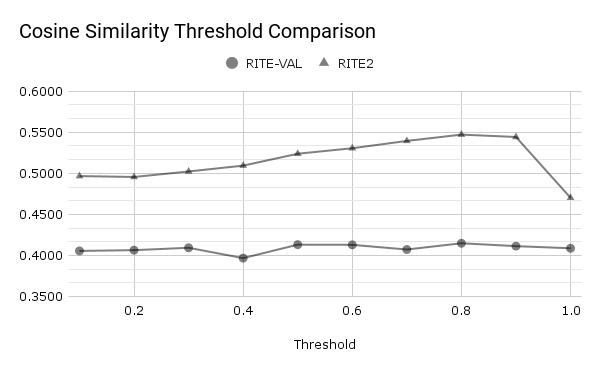
\includegraphics[width=15cm]{SimThresholdComp.png}
  \caption[Cosine Similarity Threshold Comparison]{This figure shows the trend of the performance with different cosine similarity thresholds in each dataset. The performances between 0.8 to 1.0 are much better than the other intervals, and 0.8 seems the common highest point overall.}
  \label{fig:threshold}
\end{figure}

\begin{table}[H]
  \centering
  \begin{tabular}{|R{2.5cm}|R{2.5cm}|R{2.5cm}|R{3cm}|R{2.5cm}|}
  \hline
  \multicolumn{1}{|c|}{Threshold} & \multicolumn{1}{c|}{RITE-VAL} & \multicolumn{1}{c|}{RITE2} & \multicolumn{1}{c|}{RITE-VAL-TEST} & \multicolumn{1}{c|}{RITE2-TEST} \\ \hline
  0.1 & 0.4188 & 0.4894 & 0.3455 & 0.3440 \\ \hline
  0.2 & 0.4032 & 0.4992 & 0.3314 & 0.3564 \\ \hline
  0.3 & 0.4144 & 0.5023 & 0.3223 & 0.3523 \\ \hline
  0.4 & 0.3967 & 0.5094 & 0.3210 & 0.4058 \\ \hline
  0.5 & 0.4161 & 0.5239 & 0.3041 & 0.4030 \\ \hline
  0.6 & 0.4134 & 0.5306 & 0.3137 & 0.3837 \\ \hline
  0.7 & 0.4116 & 0.5352 & 0.3109 & 0.3795 \\ \hline
  0.8 & 0.4223 & 0.5413 & 0.3419 & 0.3720 \\ \hline
  0.9 & 0.4062 & 0.5415 & 0.3137 & 0.4015 \\ \hline
  1.0 & 0.4010 & 0.5442 & 0.3510 & 0.3853 \\ \hline
  \end{tabular}
  \caption{The detailed performance of the comparison of the cosine similarity threshold arguments in the cosine similarity alignment method.}
  \label{result:threshold_comparison}
\end{table}

\paragraph{}
We concatenated the machine learning features mention in section \ref{section:ml_features} with the hidden states of the cosine similarity alignment to see the performance, the results are shown in table \ref{result:csa_nn}. Most of the performances are better than the neural network input by cosine similarity alignment only, proving that the machine learning features have benefits to the models.

\begin{table}[H]
  \centering
  \begin{tabular}{|l|R{2.5cm}|R{2.5cm}|R{3cm}|R{2.5cm}|}
  \hline
  \multicolumn{1}{|c|}{Features} & \multicolumn{1}{c|}{RITE-VAL} & \multicolumn{1}{c|}{RITE2} & \multicolumn{1}{c|}{RITE-VAL-TEST} & \multicolumn{1}{c|}{RITE2-TEST} \\ \hline
  CSA Only & 0.4062 & \textbf{0.5415} & 0.3137 & 0.4015 \\ \hline
  CSA + ML Features & \textbf{0.4283} & 0.5407 & \textbf{0.3364} & \textbf{0.4069} \\ \hline
  \end{tabular}
  \caption{Comparison of the features in the neural network.}
  \label{result:csa_nn}
\end{table}

\paragraph{}
We use the reversed labels of RITE-VAL and combined with the RITE2 as a new training dataset called RITE-Extended, the total data size increased to 1,902 and processed into the experiments. The results are shown in table \ref{result:rite_extended}, the performance does not seem to improve much, we think the scale of the increased data size is not large enough to have a huge impact on the experiments.

\begin{table}[H]
  \centering
  \begin{tabular}{|l|R{2.5cm}|R{2.5cm}|R{3cm}|R{2.5cm}|}
  \hline
  \multicolumn{1}{|c|}{Dataset} & \multicolumn{1}{c|}{RITE-VAL} & \multicolumn{1}{c|}{RITE2} & \multicolumn{1}{c|}{RITE-VAL-TEST} & \multicolumn{1}{c|}{RITE2-TEST} \\ \hline
  Original & \textbf{0.4283} & \textbf{0.5407} & 0.3364 & \textbf{0.4069} \\ \hline
  Extended & 0.4081 & 0.5204 & \textbf{0.3505} & \textbf{0.4032} \\ \hline
  \end{tabular}
  \caption{Comparison of the original RITE and the extended RITE}
  \label{result:rite_extended}
\end{table}

\subsection{Experiments with Additional NLI Datasets}
\paragraph{}
We first reproduce the performance of BERT on the MNLI dataset. In this experiment, the \texttt{bert-base-uncased} is used, the learning rate is 3e-5. After 2 epochs of training, the accuracy of the dev set is 0.8346, which is close to the original paper (0.846). Then we reproduce the same experiment of BERT on the OCNLI dataset but replace with \texttt{bert-base-chinese} model, the accuracy of the dev set is 0.7447, which is also close to the original paper (0.745).

% 成功重製以上兩個實驗的效能後,我們將相同的實驗設定套用到 CNLI 上。CNLI 的 dev set 準確率為 0.7830 而 test set 準確率為 0.7832。雖然並不如 CCL 2018 會議上最好的系統 (0.8238) 但是比第二名的系統好 (0.7828)。
\paragraph{}
After reproducing these two experiments above successfully, we applied the same experiment on the CNLI dataset. The accuracy of the dev set of CNLI is 0.7830, and the accuracy of the test set is 0.7832. Though the performance is not better than the best system in CCL 2018 which reached 0.8238, the performance is better than the second-best system (0.7828).

\paragraph{}
% 接下來,我們開始關注當 RITE 資料集做為 validation set 並使用其他大型 NLI 資料集做 pre-training 時,BERT 的效能如何。因為其他大型 NLI 資料集皆為 ECN task 而 RITE 為 BFCI task,所以我們會先用訓練資料集訓練一個 ECN Model,然後將訓練資料集的 premise 與 hypothesis 對調再進行 prediction,若對調前的 label 為 entailment 而且對調後的 prediction 也是 entailment,就將這組 sentence pair 標記為 bi-directional,由此產生 BFCI 版本的訓練資料集,再以此版本資料集作為訓練資料集。
Next, we focus on how the performance of BERT will be when the RITE dataset is validation set and using other large-scale NLI datasets as the training set. Because the task type of other large-scale NLI datasets are ECN task, but the task type of RITE is BFCI task, we need to train an ECN model first, then we swap the premise and the hypothesis of the training set and do the prediction. If the original label and the prediction of the swapped sentence pair are both ``entailment'', then we mark this sentence pair as ``bi-directional'', so we can generate the BFCI version of the dataset and use this version of the dataset as the training set.

\paragraph{}
% 首先我們以 CNLI 做為 pre-training data 並以 RITE 進行 fine-tune。
We use the CNLI dataset as the training data first, then test on RITE2 and RITE-VAL directly. The BERT model we fine-tuned is \texttt{bert-base-chinese} The result is shown in table \ref{result:bert_cnli}, we can see that the performance of the test set is much better than the best system in either Liu et al or NTCIR.

\begin{table}[H]
  \centering
  \begin{tabular}{|c|l|r|r|r|r|}
  \hline
  \multirow{2}{*}{\#} & \multicolumn{1}{c|}{\multirow{2}{*}{System}} & \multicolumn{2}{c|}{RITE-VAL} & \multicolumn{2}{c|}{RITE2} \\ \cline{3-6}
   & \multicolumn{1}{c|}{} & \multicolumn{1}{c|}{Dev} & \multicolumn{1}{c|}{Test} & \multicolumn{1}{c|}{Dev} & \multicolumn{1}{c|}{Test} \\ \hline
  1 & CNLI-Only & 0.4766 & 0.4993 & 0.5377 & 0.5950 \\ \hline
  2 & CNLI-TW & 0.5915 & 0.5146 & 0.6848 & 0.6426 \\ \hline
  3 & CNLI-CN & 0.5609 & 0.4977 & 0.6724 & 0.6293 \\ \hline
  4 & MNLI & 0.5713 & \textbf{0.5561} & 0.6919 & \textbf{0.7107} \\ \hline
  5 & OCNLI & 0.5316 & 0.5092 & 0.6710 & 0.5884 \\ \hline
  6 & MNLI-CNLI & 0.5811 & \textbf{0.5650} & 0.6952 & 0.6955 \\ \hline
  7 & Mixed-NLI & 0.5895 & \textbf{0.5592} & 0.6880 & \textbf{0.7036} \\ \hline
  8 & MNLI + ML Features & 0.5216 & 0.5301 & 0.6697 & \textbf{0.7032} \\ \hline
  \end{tabular}
  \caption{Results of the BERT that train with the different datasets.}
  \label{result:bert_compare}
\end{table}

\begin{table}[H]
  \centering
  \begin{tabular}{|l|r|r|r|r|r|}
  \hline
   & \multicolumn{1}{c|}{B-F1} & \multicolumn{1}{c|}{F-F1} & \multicolumn{1}{c|}{C-F1} & \multicolumn{1}{c|}{I-F1} & \multicolumn{1}{c|}{Macro F1} \\ \hline
  RITE-VAL & 0.7024 & 0.5022 & 0.4863 & 0.2157 & 0.4766 \\ \hline
  RITE-VAL-TEST & 0.6110 & 0.5506 & 0.5219 & 0.3135 & 0.4993 \\ \hline
  RITE2 & 0.5443 & 0.7003 & 0.4158 & 0.4902 & 0.5377 \\ \hline
  RITE2-TEST & 0.6797 & 0.6667 & 0.5035 & 0.5303 & 0.5950 \\ \hline
  \end{tabular}
  \caption{Results of BERT that train with CNLI and directly test with RITE.}
  \label{result:bert_cnli}
\end{table}

\paragraph{}
% 藉由上個實驗的成功,我們進一步的將 RITE 切成 10-fold 並納入 fine-tune 的環節,我們將 CNLI 訓練出來的模型透過每個 fold 的 training set 再進行一次訓練,並測試該 fold 的 test set,最後將每個 fold 的測試集結果合併在一起進算 micro f1。得到的結果如表 x,其效能有大幅度的提昇。
With the success of the previous experiment, we split the RITE dataset into fixed 10-folds and bring it into the fine-tuning. We use the training set of each fold to train after the model that trained by the CNLI-TW dataset and test on the test set of the fold, then we merge the results of all folds and calculate the micro f1-score. The result is shown in table \ref{result:bert_cnli_transfer}, the performance has a huge improvement.

\begin{table}[H]
  \centering
  \begin{tabular}{|l|r|r|r|r|r|}
  \hline
   & \multicolumn{1}{c|}{B-F1} & \multicolumn{1}{c|}{F-F1} & \multicolumn{1}{c|}{C-F1} & \multicolumn{1}{c|}{I-F1} & \multicolumn{1}{c|}{Macro F1} \\ \hline
  RITE-VAL & 0.7384 & 0.6754 & 0.6224 & 0.3299 & 0.5915 \\ \hline
  RITE-VAL-TEST & 0.6084 & 0.6172 & 0.5764 & 0.2565 & 0.5146 \\ \hline
  RITE2 & 0.6827 & 0.8444 & 0.5493 & 0.6627 & 0.6848 \\ \hline
  RITE2-TEST & 0.7140 & 0.7393 & 0.5315 & 0.5856 & 0.6426 \\ \hline
  \end{tabular}
  \caption{Results of the BERT that train with CNLI-TW and fine-tune with RITE.}
  \label{result:bert_cnli_transfer}
\end{table}

\paragraph{}
We also compared the performance between CNLI and CNLI-TW, the result of CNLI is shown in table \ref{result:bert_cnli_cn}. Compare to table \ref{result:bert_cnli_transfer}, we can see that the performance of CNLI-TW is better than CNLI, so we think the dataset composed of Traditional Chinese characters is more suitable for RITE, even though the dataset is augmented from the translation tool.

\begin{table}[H]
  \centering
  \begin{tabular}{|l|r|r|r|r|r|}
  \hline
   & \multicolumn{1}{c|}{B-F1} & \multicolumn{1}{c|}{F-F1} & \multicolumn{1}{c|}{C-F1} & \multicolumn{1}{c|}{I-F1} & \multicolumn{1}{c|}{Macro F1} \\ \hline
  RITE-VAL & 0.6881 & 0.6424 & 0.5893 & 0.3238 & 0.5609 \\ \hline
  RITE-VAL-TEST & 0.5316 & 0.6077 & 0.5579 & 0.2936 & 0.4977 \\ \hline
  RITE2 & 0.6718 & 0.8408 & 0.5167 & 0.6605 & 0.6724 \\ \hline
  RITE2-TEST & 0.6796 & 0.7336 & 0.4811 & 0.6228 & 0.6293 \\ \hline
  \end{tabular}
  \caption{Results of the BERT that train with CNLI-CN and fine-tune with RITE.}
  \label{result:bert_cnli_cn}
\end{table}

\paragraph{}
% 根據上述的實驗結果顯示,資料集的規模對模型效能有巨大的影響,而正確的 fine-tune 步驟也起了關鍵的作用。所以我們下一步決定嘗試使用 MNLI 資料集來訓練 BERT 的跨語言模型,並用相同的步驟以 RITE 進行 fine-tune。
According to the results of the above experiments, the scale of the training datasets has a huge impact on performance, and the correct steps of fine-tuning are also the key part. So we decided to use the MNLI dataset to train the cross-lingual BERT model (\texttt{bert-multilingual-cased}) and fine-tuned with the RITE dataset with the same steps. The result is shown in table \ref{result:bert_mnli_transfer}, we can see the performance has a little improvement.

\begin{table}[H]
  \centering
  \begin{tabular}{|l|r|r|r|r|r|}
  \hline
   & \multicolumn{1}{c|}{B-F1} & \multicolumn{1}{c|}{F-F1} & \multicolumn{1}{c|}{C-F1} & \multicolumn{1}{c|}{I-F1} & \multicolumn{1}{c|}{Macro F1} \\ \hline
  RITE-VAL & 0.7478 & 0.6689 & 0.5567 & 0.3119 & 0.5713 \\ \hline
  RITE-VAL-TEST & 0.6137 & 0.6291 & 0.6122 & 0.3696 & 0.5561 \\ \hline
  RITE2 & 0.6867 & 0.8640 & 0.5247 & 0.6920 & 0.6919 \\ \hline
  RITE2-TEST & 0.7834 & 0.7881 & 0.5757 & 0.6955 & 0.7107 \\ \hline
  \end{tabular}
  \caption{Results of the BERT that train with MNLI and fine-tune with RITE.}
  \label{result:bert_mnli_transfer}
\end{table}

\paragraph{}
% 我們同樣進行了以 OCNLI 為訓練資料的實驗,OCNLI 的句子品質相較於 CNLI 而言較高一點,但其資料規模並不如 CNLI。以同樣的方法進行實驗之後,其實驗結果如表。結果顯示,以 OCNLI 為訓練集的實驗,無論在 RITE2 或 RITE-VAL 的實驗上,效能皆不如以 CNLI 作為訓練集的實驗。
We also do the experiment that uses OCNLI as the training set. The quality of sentences of OCNLI seems higher than CNLI, but the scale of data size is lower. The result is shown in table \ref{result:bert_ocnli_transfer}, and we can see, compared to the experiment of CNLI, the performance is lower no matter on RITE2 or RITE-VAL.

\begin{table}[H]
  \centering
  \begin{tabular}{|l|r|r|r|r|r|}
  \hline
   & \multicolumn{1}{c|}{B-F1} & \multicolumn{1}{c|}{F-F1} & \multicolumn{1}{c|}{C-F1} & \multicolumn{1}{c|}{I-F1} & \multicolumn{1}{c|}{Macro F1} \\ \hline
  RITE-VAL & 0.6870 & 0.6667 & 0.4948 & 0.2778 & 0.5316 \\ \hline
  RITE-VAL-TEST & 0.5608 & 0.6091 & 0.5517 & 0.3153 & 0.5092 \\ \hline
  RITE2 & 0.6416 & 0.8406 & 0.5209 & 0.6810 & 0.6710 \\ \hline
  RITE2-TEST & 0.6488 & 0.7120 & 0.4000 & 0.5928 & 0.5884 \\ \hline
  \end{tabular}
  \caption{Results of the BERT that train with OCNLI and fine-tune with RITE.}
  \label{result:bert_ocnli_transfer}
\end{table}

\paragraph{}
% 我們試著將 CSA 與 ML Features 這兩種方法與 BERT 模型做結合。與 CSA 結合的部份,我們先透過一層 RNN 進行 Encoding 然後與 BERT Hidden State 拼接在一起進行輸出,而 ML Features 的部份則是直接拼接並進行輸出,最後還有將三者做結合的實驗,並以 CNLI 做為 benchmark。其實驗結果如表,從 RITE-VAL 的角度來看,加入 CSA 與 ML Features 的做法並沒有帶來正面的提昇,而從 RITE2 的角度而言,效能的提昇也是相當微幅。可見 BERT 所能學習到的特徵表示是相當深入的。
We try to combine the BERT model with the CSA and the ML features to see how these features will impact the performance. We use the CNLI dataset as the benchmark. In the CSA combination, we first encode the CSA features with an RNN layer and concatenated them with BERT hidden states to output. In the ML features, we simply concatenated the features with BERT hidden states. Finally, we concatenated three of them for comparison. The results are shown in table \ref{result:bert_csa_mlft_comparison}. No matter the CSA and ML features or both of them have no positive improvement to the RITE-VAL, and only have a little improvement to the RITE2. We can see that the feature representation that the BERT model can learn is quite in-depth.

\begin{table}[H]
  \centering
  \begin{tabular}{|l|R{2.5cm}|R{2.5cm}|R{2.5cm}|R{2.5cm}|}
  \hline
  \multicolumn{1}{|c|}{System} & \multicolumn{1}{c|}{RITE-VAL} & \multicolumn{1}{c|}{RITE2} & \multicolumn{1}{c|}{RITE-VAL-TEST} & \multicolumn{1}{c|}{RITE2-TEST} \\ \hline
  Original & 0.4766 & 0.5377 & \textbf{0.4993} & 0.5950 \\ \hline
  ft. MLFT & 0.4717 & 0.5390 & 0.4502 & 0.6006 \\ \hline
  ft. CSA & \textbf{0.4853} & \textbf{0.5432} & 0.4687 & \textbf{0.6058} \\ \hline
  ft. MLFT + CSA & \textbf{0.4853} & 0.4857 & \textbf{0.5407} & 0.6027 \\ \hline
  \end{tabular}
  \caption{Comparison of the CSA and the ML features with BERT. Using the CNLI dataset as the benchmark, ``MLFT'' means the ML features.}
  \label{result:bert_csa_mlft_comparison}
\end{table}

\paragraph{}
% 因為跨語言實驗的提昇,所以我們想試試看混合語言的效果如何。我們使用兩種方法來進行混合語言的實驗:第一個是先用 MNLI 訓練,再用 CNLI 訓練:第二個是將 MNLI 與 CNLI 的訓練集混合在一起變成新的訓練資料集,我們稱之為 Mixed-NLI,然後進行訓練。前者的實驗結果如表X,後者的實驗結果如表Y。與使用 MNLI 做為訓練資料的實驗相比,效能的改進幅度相當的小,甚至是降低了一點,但差距幾乎都在 0.1% 以內。所以我們認為在資料規模超過 MNLI 之後能獲得的效能提昇相當有限。
Due to the improvement of the cross-lingual experiment, we want to know the performance of the mix-lingual. We use two ways to achieve the mix-lingual experiment. The first is to train with MNLI, and then train with CNLI. The second is to mix MNLI and CNLI into a new training set we called Mixed-NLI. The results are shown in table \ref{result:bert_mnli_cnli} and table \ref{result:bert_mixed_nli}, as we can see, compared to the experiment of MNLI, both of the improvement of the two experiments are quite small and even decreases on RITE2, but the differences are within 0.1\%. So we think when the scale of data size is over than the size of MNLI, the improvement of performance is quite limited.

\begin{table}[H]
  \centering
  \begin{tabular}{|l|r|r|r|r|r|}
  \hline
   & \multicolumn{1}{c|}{B-F1} & \multicolumn{1}{c|}{F-F1} & \multicolumn{1}{c|}{C-F1} & \multicolumn{1}{c|}{I-F1} & \multicolumn{1}{c|}{Macro F1} \\ \hline
  RITE-VAL & 0.7522 & 0.6839 & 0.5895 & 0.2991 & 0.5811 \\ \hline
  RITE-VAL-TEST & 0.6291 & 0.6365 & 0.6163 & 0.3780 & 0.5650 \\ \hline
  RITE2 & 0.6906 & 0.8551 & 0.5520 & 0.6830 & 0.6952 \\ \hline
  RITE2-TEST & 0.7689 & 0.7748 & 0.5662 & 0.6721 & 0.6955 \\ \hline
  \end{tabular}
  \caption{Results of the BERT that train with MNLI first then train with CNLI, and fine-tune with RITE.}
  \label{result:bert_mnli_cnli}
\end{table}

\begin{table}[H]
  \centering
  \begin{tabular}{|l|r|r|r|r|r|}
  \hline
   & \multicolumn{1}{c|}{B-F1} & \multicolumn{1}{c|}{F-F1} & \multicolumn{1}{c|}{C-F1} & \multicolumn{1}{c|}{I-F1} & \multicolumn{1}{c|}{Macro F1} \\ \hline
  RITE-VAL & 0.7505 & 0.6537 & 0.5866 & 0.3670 & 0.5895 \\ \hline
  RITE-VAL-TEST & 0.6326 & 0.6268 & 0.6042 & 0.3731 & 0.5592 \\ \hline
  RITE2 & 0.6962 & 0.8455 & 0.5322 & 0.6779 & 0.6880 \\ \hline
  RITE2-TEST & 0.7731 & 0.7936 & 0.5604 & 0.6875 & 0.7036 \\ \hline
  \end{tabular}
  \caption{Results of the BERT that train with Mixed-NLI and fine-tune with RITE.}
  \label{result:bert_mixed_nli}
\end{table}

\paragraph{}
We also feed the machine learning features mentioned in section \ref{section:ml_features} into BERT, concatenating with the pooled outputs of BERT. The result is shown in table \ref{result:bert_mnli_ft}. However, the performance is not increased, so we think the traditional feature is not helpful to the deep learning models of this experiment.

\begin{table}[H]
  \centering
  \begin{tabular}{|l|r|r|r|r|r|}
  \hline
   & \multicolumn{1}{c|}{B-F1} & \multicolumn{1}{c|}{F-F1} & \multicolumn{1}{c|}{C-F1} & \multicolumn{1}{c|}{I-F1} & \multicolumn{1}{c|}{Macro F1} \\ \hline
  RITE-VAL & 0.7394 & 0.6000 & 0.5387 & 0.2083 & 0.5216 \\ \hline
  RITE-VAL-TEST & 0.6245 & 0.6135 & 0.5709 & 0.3113 & 0.5301 \\ \hline
  RITE2 & 0.6690 & 0.8378 & 0.4913 & 0.6805 & 0.6697 \\ \hline
  RITE2-TEST & 0.7734 & 0.7829 & 0.5637 & 0.6927 & 0.7032 \\ \hline
  \end{tabular}
  \caption{Results of the BERT that train with MNLI and fine-tune with RITE, using ML Features.}
  \label{result:bert_mnli_ft}
\end{table}

\subsection{Experiments with Pseudo Training Data}
% 描述 RITE Extended 關於 Training Data Size 的探討
\paragraph{}
We try to use the information of RITE-VAL reversed labels to expand our training source, in purpose to advanced discuss the impact of training data size on the performance. The result is shown in table \ref{result:ml_expand}. As we can see, when the data size get increased, the performance of simple DNN get much better.

\begin{table}
  \centering
  \begin{tabular}{|l|R{2.5cm}|R{2.5cm}|R{2.5cm}|R{2.5cm}|}
  \hline
  Training Source & \multicolumn{2}{c|}{RITE-VAL-REV} & \multicolumn{2}{c|}{RITE-VAL-REV-2} \\ \hline
  Classifier & \multicolumn{1}{c|}{SVM} & \multicolumn{1}{c|}{Simple DNN} & \multicolumn{1}{c|}{SVM} & \multicolumn{1}{c|}{Simple DNN} \\ \hline
  Validation Target & \multicolumn{4}{c|}{RITE-VAL} \\ \hline
  all & 0.3834 & 0.4483 & 0.4011 & \textbf{0.4640} \\ \hline
  all - lex & 0.3704 & 0.4374 & 0.4047 & 0.4494 \\ \hline
  all - syn & 0.3747 & 0.3977 & 0.4045 & 0.4037 \\ \hline
  all - wn & \textbf{0.3898} & \textbf{0.4486} & \textbf{0.4122} & 0.4554 \\ \hline
  all - cl & 0.3498 & 0.4416 & 0.3978 & 0.4554 \\ \hline
  Validation Target & \multicolumn{4}{c|}{RITE2} \\ \hline
  all & \textbf{0.4528} & \textbf{0.5359} & 0.5177 & 0.5723 \\ \hline
  all - lex & 0.4327 & 0.5191 & 0.4868 & 0.5498 \\ \hline
  all - syn & 0.4173 & 0.4775 & 0.4997 & 0.5147 \\ \hline
  all - wn & 0.4431 & 0.5252 & 0.4941 & 0.5700 \\ \hline
  all - cl & 0.4368 & 0.5358 & \textbf{0.5410} & \textbf{0.5792} \\ \hline
  Validation Target & \multicolumn{4}{c|}{RITE-VAL-TEST} \\ \hline
  all & \textbf{0.3872} & 0.3862 & 0.3900 & 0.4020 \\ \hline
  all - lex & 0.3165 & 0.3789 & 0.3570 & 0.3857 \\ \hline
  all - syn & 0.3125 & 0.3060 & 0.3227 & 0.3182 \\ \hline
  all - wn & 0.3683 & 0.3785 & \textbf{0.3903} & 0.3941 \\ \hline
  all - cl & 0.3865 & \textbf{0.3902} & 0.3899 & \textbf{0.4138} \\ \hline
  Validation Target & \multicolumn{4}{c|}{RITE2-TEST} \\ \hline
  all & 0.4157 & 0.4287 & 0.4365 & \textbf{0.4742} \\ \hline
  all - lex & 0.4114 & 0.4189 & 0.4416 & 0.4394 \\ \hline
  all - syn & 0.4315 & 0.4215 & 0.4318 & 0.4457 \\ \hline
  all - wn & \textbf{0.4354} & 0.4252 & \textbf{0.4618} & 0.4663 \\ \hline
  all - cl & 0.4249 & \textbf{0.4266} & 0.4497 & 0.4717 \\ \hline
  \end{tabular}
  \caption{Results of SVM and simple DNN comparison using expanded training data.}
  \label{result:ml_expand}
\end{table}

% [描述 Pseudo Training Data Size 的實驗] 我們將 Pseudo Training Data 與 RNN 的實驗做結合,並觀察不同資料量對於系統效能的影響,並將系統效能與資料量之間的關係畫成曲線圖,其結果如圖,可見資料量與系統效能間有正相關,但在資料量超過 100k 之後就開始有邊際效應出現,雖然效能還是有所提昇,但提昇的幅度並沒有很大。
\paragraph{}
We put the pseudo training data into the experiments of RNN and observe the impact of the system performance to each different scale of data size, then plot the relation between data size and performance. The result is shown in figure \ref{fig:pseudo_datasize}, we can see the positive correlation between data size and performance, but there is a marginal effect when the scale of data size comes over 100 thousand, the performance has improved but the improvement is not huge.

\begin{figure}[H]
  \centering
  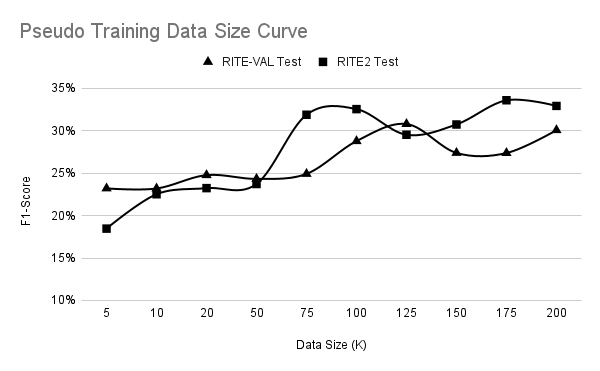
\includegraphics[width=15cm]{PseudoTrainingDataSizeCurve.png}
  \caption[Pseudo Training Data Size Curve]{The relationship between pseudo training data size and the performance of the RNN model.}
  \label{fig:pseudo_datasize}
\end{figure}

% 將 CNLI 放入 RNN 的實驗

\begin{table}[H]
  \centering
  \begin{tabular}{|l|R{2.5cm}|R{2.5cm}|R{3cm}|R{2.5cm}|}
  \hline
  \multicolumn{1}{|c|}{System} & \multicolumn{1}{c|}{RITE-VAL} & \multicolumn{1}{c|}{RITE2} & \multicolumn{1}{c|}{RITE-VAL-TEST} & \multicolumn{1}{c|}{RITE2-TEST} \\ \hline
  RAD & 0.3314 & 0.2849 & 0.2710 & 0.2926 \\ \hline
  RAD + CSA + MLFT & \textbf{0.4601} & \textbf{0.4847} & \textbf{0.3762} & \textbf{0.4643} \\ \hline
  \end{tabular}
  \caption{Using CNLI as training data in the RNN experiments.}
  \label{result:rnn_cnli}
\end{table}

% 我們將虛擬訓練資料章節所產生的虛擬資料用來訓練 BERT,並且以 RITE 資料集做微調,也嘗試將虛擬資料與 CNLI 資料集混合在一起做為不同的訓練資料來測試其效能,其結果如表。在規則式虛擬資料與 CNLI 資料集混合的實驗中,其效能高於只用 CNLI 資料集做為訓練資料的實驗。
\paragraph{}
We use the pseudo training data mentioned in section \ref{section:pseudo} as the pretraining dataset to train BERT and fine-tuned with the RITE dataset, we also try to mix the pseudo dataset with the CNLI dataset to see the performance. The result is shown in table \ref{result:pseudo_nli_bert}. We can see the performance of the rule-based pseudo dataset is better than the GPT2 pseudo dataset, and the performance of rule-based pseudo dataset mixed with the CNLI dataset is better than the performance of the CNLI dataset.

\begin{table}[H]
  \centering
  \begin{tabular}{|l|R{2cm}|R{2cm}|R{2cm}|R{2cm}|}
  \hline
  \multicolumn{1}{|c|}{\multirow{2}{*}{Dataset}} & \multicolumn{2}{c|}{RITE-VAL} & \multicolumn{2}{c|}{RITE2} \\ \cline{2-5}
  \multicolumn{1}{|c|}{} & \multicolumn{1}{c|}{Dev} & \multicolumn{1}{c|}{Test} & \multicolumn{1}{c|}{Dev} & \multicolumn{1}{c|}{Test} \\ \hline
  Rule-Based Pseudo-NLI & 0.5524 & 0.4257 & 0.6541 & \textbf{0.5777} \\ \hline
  GPT2 Pseudo-NLI & 0.5156 & 0.4210 & 0.6283 & 0.5378 \\ \hline
  Half Pseudo-NLI & 0.5255 & \textbf{0.4276} & 0.6440 & 0.5462 \\ \hline
  All Pseudo-NLI & 0.5258 & 0.4440 & 0.6695 & 0.5659 \\ \hline
  Rule-Based Pseudo-NLI + CNLI & 0.5992 & \textbf{0.5423} & 0.6908 & \textbf{0.6710} \\ \hline
  GPT2 Pseudo-NLI + CNLI & 0.5964 & 0.5364 & 0.6687 & 0.6409 \\ \hline
  CNLI & 0.5915 & 0.5146 & 0.6848 & 0.6426 \\ \hline
  \end{tabular}
  \caption{Results of the BERT that train with Pseudo-NLI and fine-tune with RITE.}
  \label{result:pseudo_nli_bert}
\end{table}

\section{Conclusion} \label{section:conclusion}
\paragraph{}
Here is the conclusion.

\end{spacing}
% \bibliography{main}
% \bibliographystyle{apa}
\printbibliography
\end{CJK*}
\end{document}

% Reference 要附上期刊集數頁數等 (journal, volume, pages)
